%============================================================
%  Capitolo 3 – Activation Functions
%============================================================
\chapter{Activation Functions}
\label{ch:activation-functions}

Le \textbf{funzioni di attivazione} sono il cuore della non-linearità nelle reti neurali.
Senza di esse, una rete a più strati si ridurrebbe a una semplice trasformazione lineare,
indipendentemente dalla profondità \citep{bishop2024}.
Come osserva Canziani nelle note NYU-DL, ogni layer di una rete tradizionale alterna
un blocco \emph{lineare} $\mathbf{s}_{k+1} = W_k \mathbf{z}_k$ a un blocco \emph{non lineare}
$\mathbf{z}_k = h(\mathbf{s}_k)$, dove $h$ è appunto la funzione di attivazione.
La scelta di $h$ influenza profondamente la velocità di convergenza, la stabilità
del gradiente e le capacità espressive della rete.

%------------------------------------------------------------
\section{Il Problema del Vanishing Gradient}
\label{sec:vanishing-gradient}

Il principale limite delle funzioni di attivazione \textbf{saturanti} (es.\ Sigmoid,
Tanh) è il cosiddetto \textbf{vanishing gradient problem}.
La retropropagazione moltiplica gradienti attraverso ogni layer: se ogni fattore è
$\ll 1$, il segnale si azzera esponenzialmente procedendo verso i layer iniziali.

Per la Sigmoid, il gradiente massimo è:
\begin{equation}
  \max_x \frac{\partial\,\sigma(x)}{\partial x}
  = \frac{1}{4} = 0{,}25 \qquad \text{(raggiunto in } x=0\text{)},
\end{equation}
e si avvicina a zero sia per $x \to +\infty$ sia per $x \to -\infty$.
In una rete con $L$ layer, il gradiente che torna al primo layer scala come
$(0{,}25)^L$: già per $L=10$ si ottiene $\approx 10^{-6}$.

\begin{figure}[H]
  \centering
  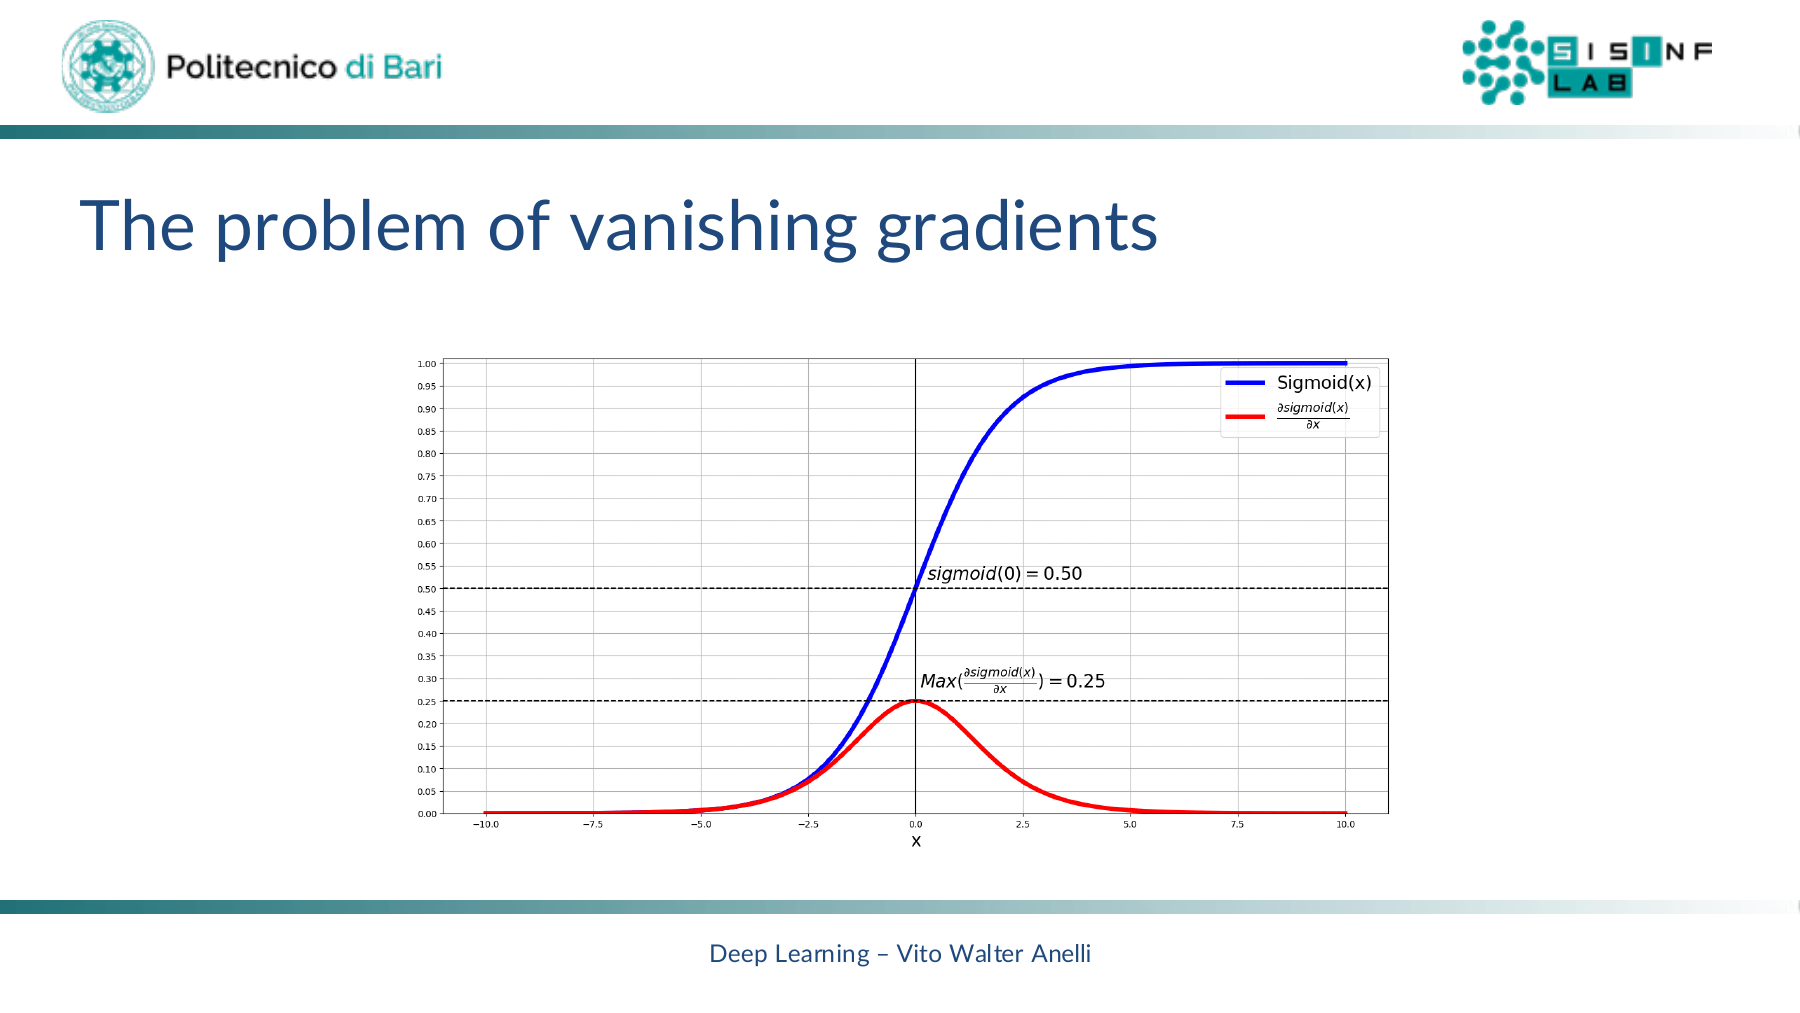
\includegraphics[width=0.82\linewidth]{figures/af03_vanishing_gradient.png}
  \caption{Sigmoid e sua derivata. Il valore $\sigma(0)=0{,}5$ è il punto di inflessione
           e il gradiente massimo è $0{,}25$. Per input molto grandi o molto piccoli
           la derivata tende a zero, bloccando il flusso del gradiente nei layer
           profondi.}
  \label{fig:vanishing_gradient}
\end{figure}

La soluzione più efficace è passare a funzioni \textbf{non saturanti} per i layer
interni, riservando funzioni saturanti solo all'output quando la struttura del
problema lo richiede (es.\ classificazione binaria, gating nelle LSTM).

%------------------------------------------------------------
\section{Panoramica: Saturating vs Non-Saturating}
\label{sec:overview-activations}

\begin{figure}[H]
  \centering
  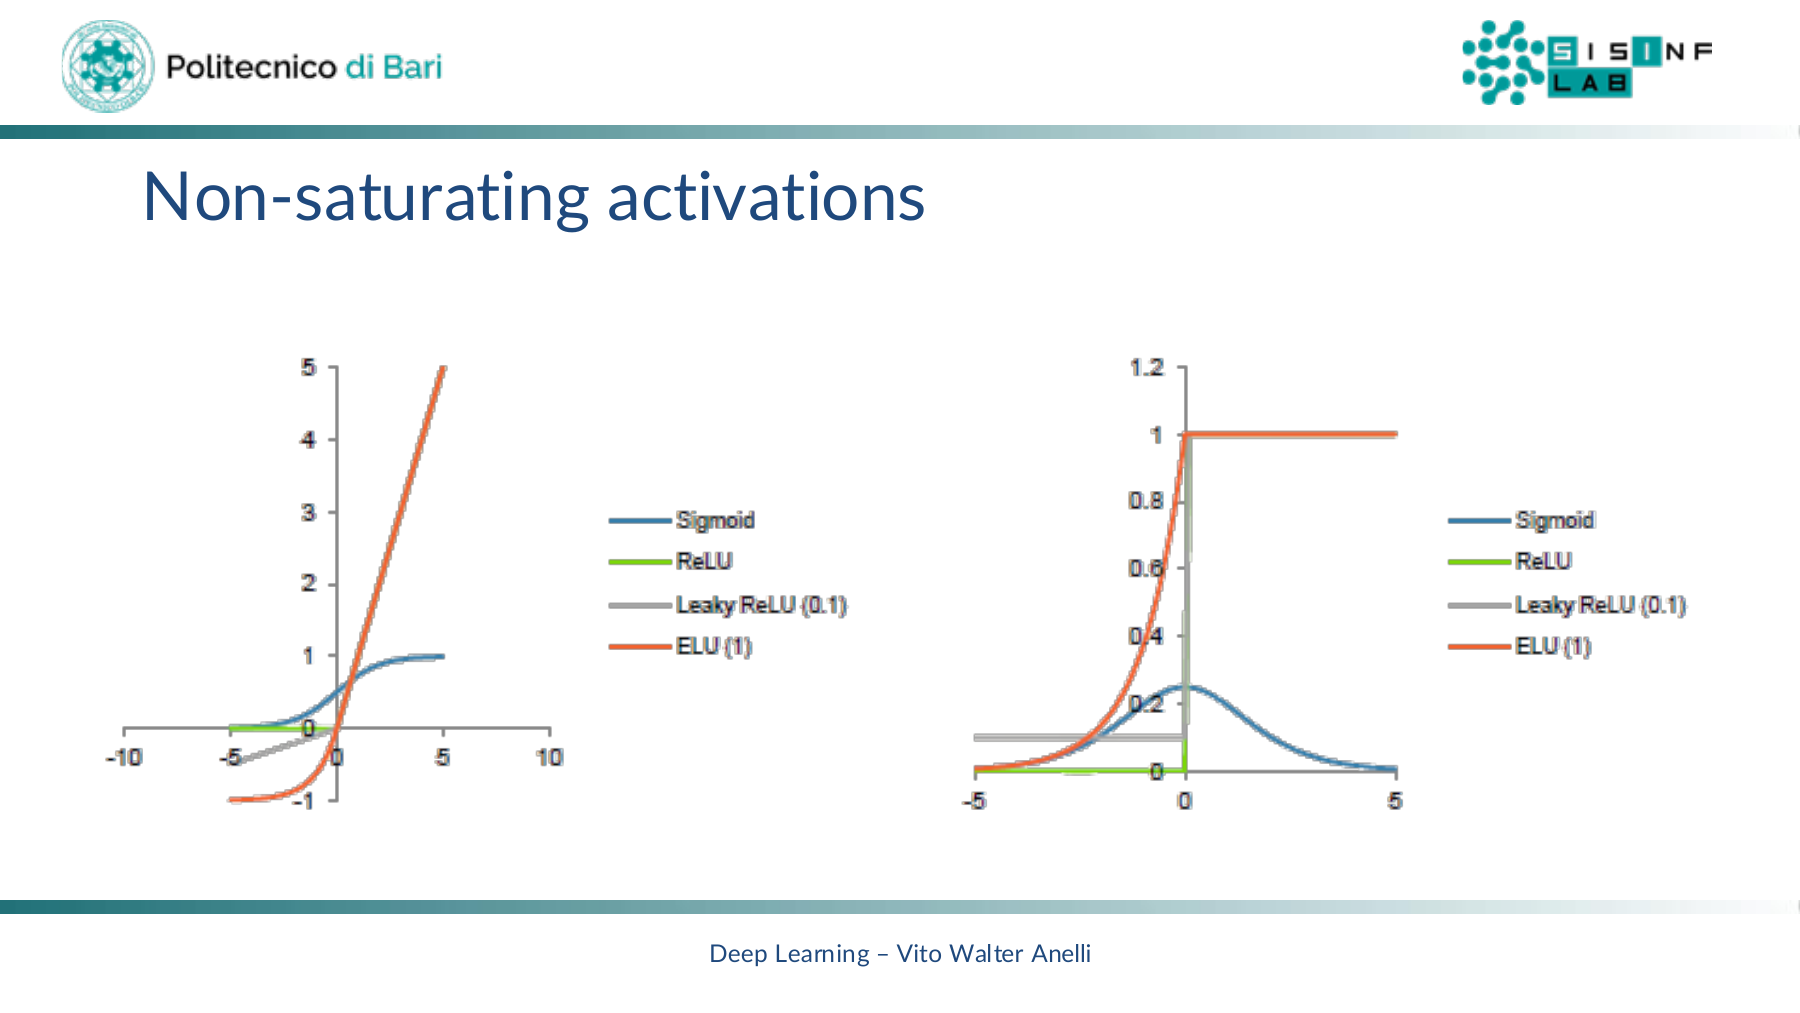
\includegraphics[width=0.90\linewidth]{figures/af03_nonsaturating_overview.png}
  \caption{Confronto visivo tra funzioni di attivazione saturanti e non saturanti
           (Sigmoid, ReLU, Leaky ReLU, ELU) nelle loro curve e nelle rispettive derivate.
           Le funzioni non saturanti mantengono un gradiente costante nella regione
           positiva, risolvendo il vanishing gradient.}
  \label{fig:nonsaturating_overview}
\end{figure}

%------------------------------------------------------------
\section{Famiglia ReLU}
\label{sec:relu-family}

\subsection{ReLU -- \texttt{nn.ReLU()}}
\label{subsec:relu}

La \textbf{Rectified Linear Unit} (ReLU) è oggi la funzione di attivazione di
default per i layer nascosti delle reti profonde \citep{bishop2024}:

\begin{equation}
  \operatorname{ReLU}(x) = (x)^{+} = \max(0, x).
\end{equation}

\begin{figure}[H]
  \centering
  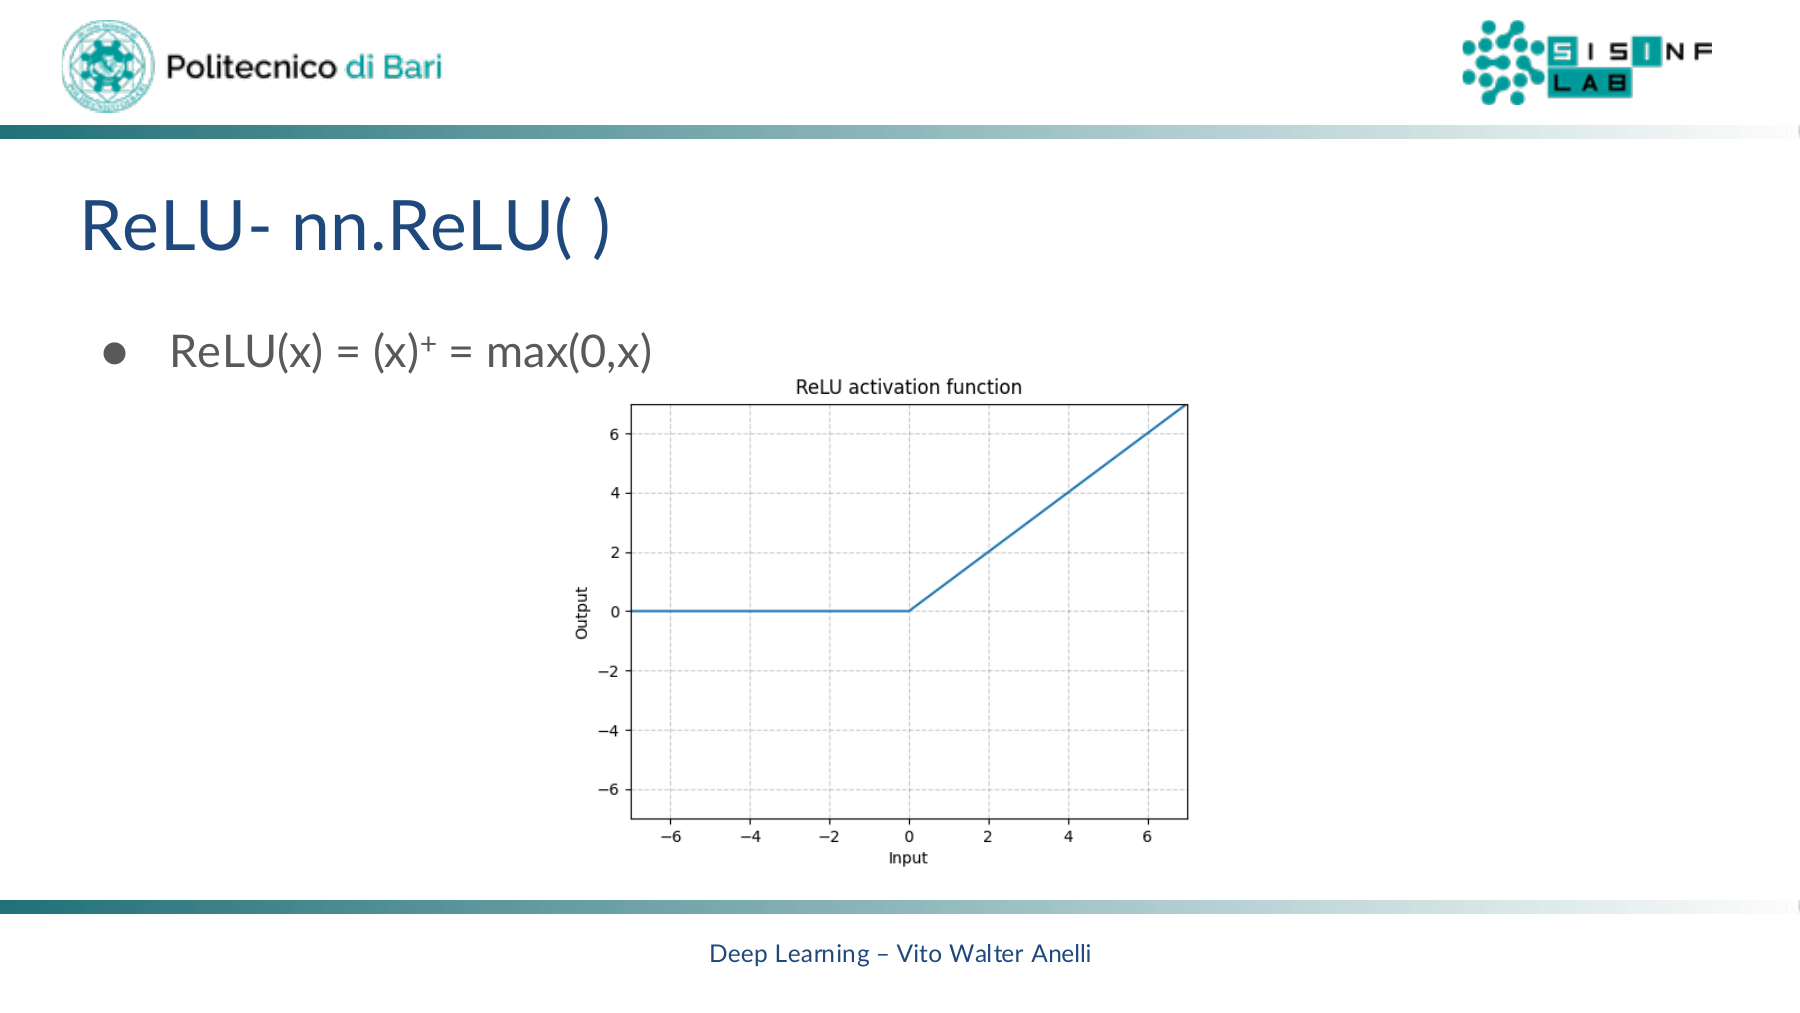
\includegraphics[width=0.72\linewidth]{figures/af03_relu.png}
  \caption{ReLU: uscita identità per $x \geq 0$, zero per $x < 0$.
           La derivata è discontinua in $x=0$ ma il gradiente è $1$ per tutti
           gli input positivi, eliminando completamente il vanishing gradient
           nel ramo attivo.}
  \label{fig:relu}
\end{figure}

\paragraph{Proprietà chiave.}
\begin{itemize}
  \item \textbf{Efficienza computazionale}: riduce a un semplice confronto con zero.
  \item \textbf{Gradiente non saturante}: la derivata è $1$ per $x>0$, evitando
        il vanishing gradient.
  \item \textbf{Sparsità}: i neuroni con input negativo producono esattamente zero,
        inducendo rappresentazioni sparse che migliorano la generalizzazione.
  \item \textbf{Dead ReLU problem}: se un neurone riceve input sempre negativi
        (es.\ dopo un grande aggiornamento del gradiente), il suo gradiente sarà
        sempre zero e il neurone cessa di apprendere. Le varianti seguenti
        mitigano questo problema.
\end{itemize}

\subsection{Leaky ReLU -- \texttt{nn.LeakyReLU()}}
\label{subsec:leaky-relu}

\begin{equation}
  \operatorname{LeakyReLU}(x) =
  \begin{cases}
    x,                                  & \text{se } x \geq 0 \\
    a_{\text{negative\_slope}} \times x, & \text{altrimenti}
  \end{cases}
\end{equation}

dove $a_{\text{negative\_slope}}$ è una piccola costante (tipicamente $0{,}01$).

\begin{figure}[H]
  \centering
  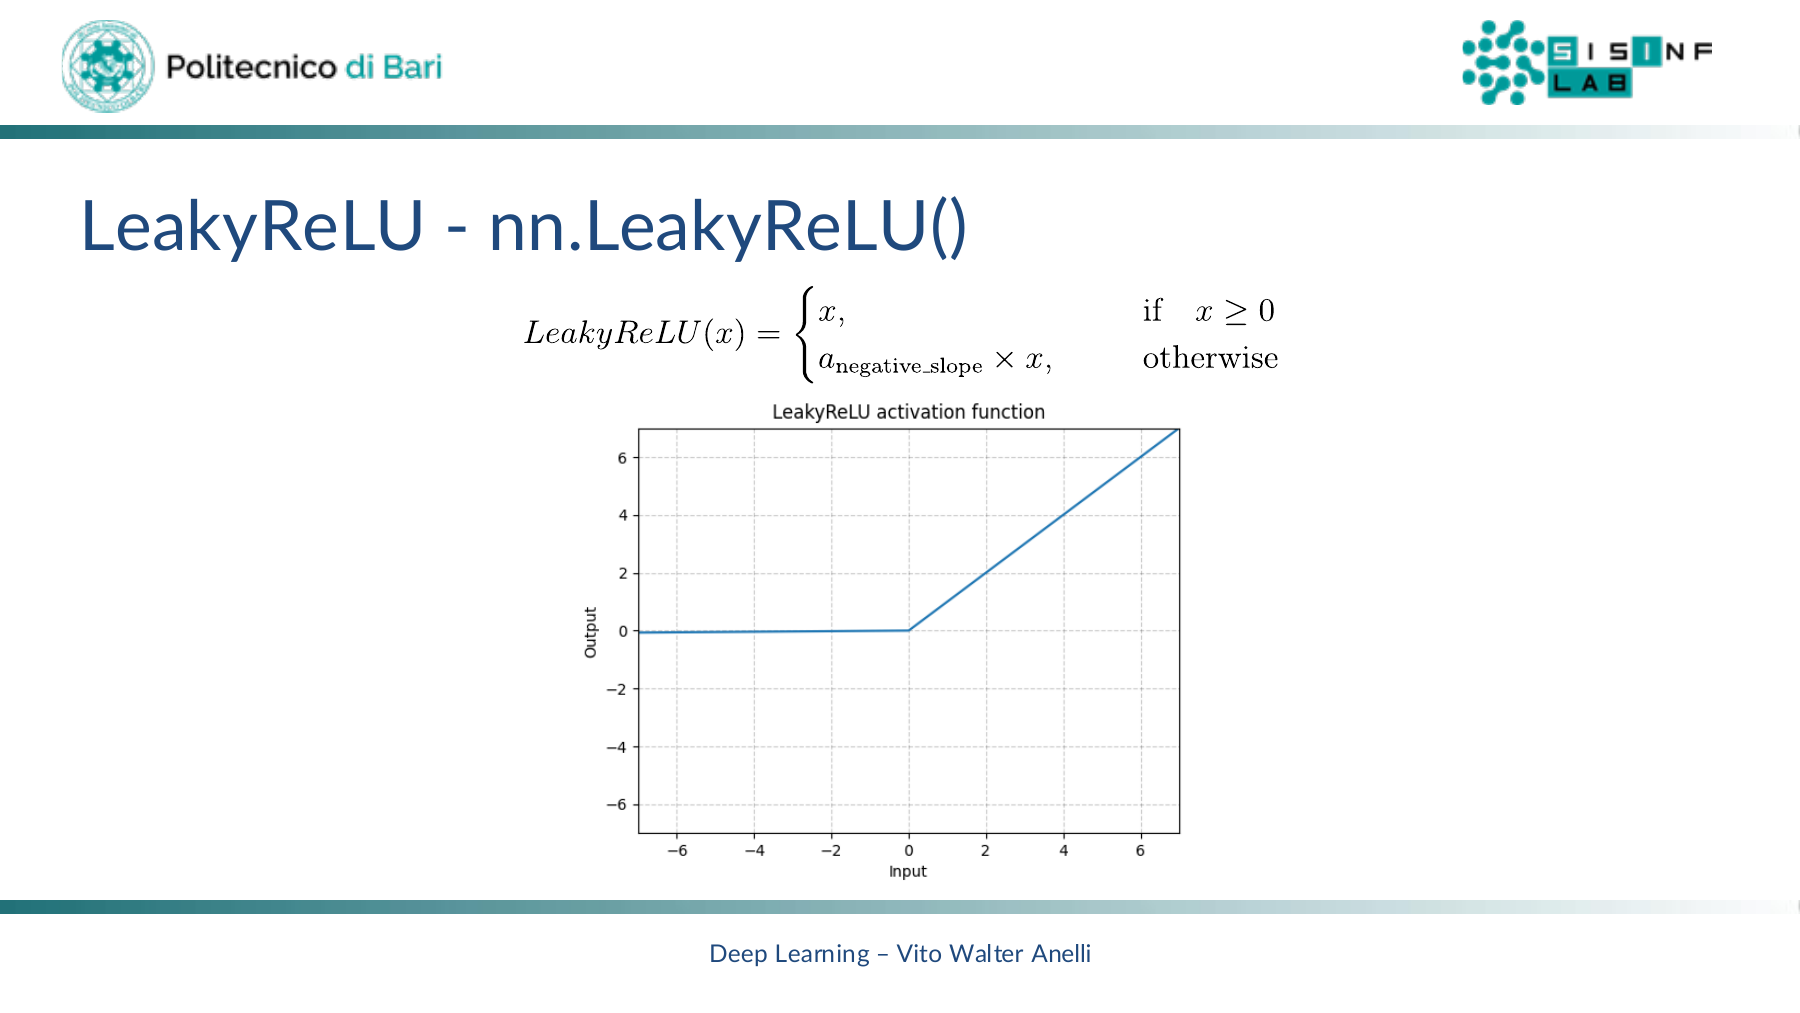
\includegraphics[width=0.72\linewidth]{figures/af03_leaky_relu.png}
  \caption{Leaky ReLU: introduce una piccola pendenza nella regione negativa
           ($a_{\text{neg}}=0{,}1$ nella figura), consentendo al gradiente di
           fluire anche per neuroni con input negativo e risolvendo il
           \emph{dead neuron} problem.}
  \label{fig:leaky_relu}
\end{figure}

Rispetto a ReLU, Leaky ReLU garantisce un gradiente non nullo anche per $x<0$,
mantenendo i neuroni attivi durante l'intero training.
Il coefficiente $a$ è fisso e scelto prima del training.

\subsection{PReLU -- \texttt{nn.PReLU()}}
\label{subsec:prelu}

\begin{equation}
  \operatorname{PReLU}(x) =
  \begin{cases}
    x,  & \text{se } x \geq 0 \\
    ax, & \text{altrimenti}
  \end{cases}
\end{equation}

\begin{figure}[H]
  \centering
  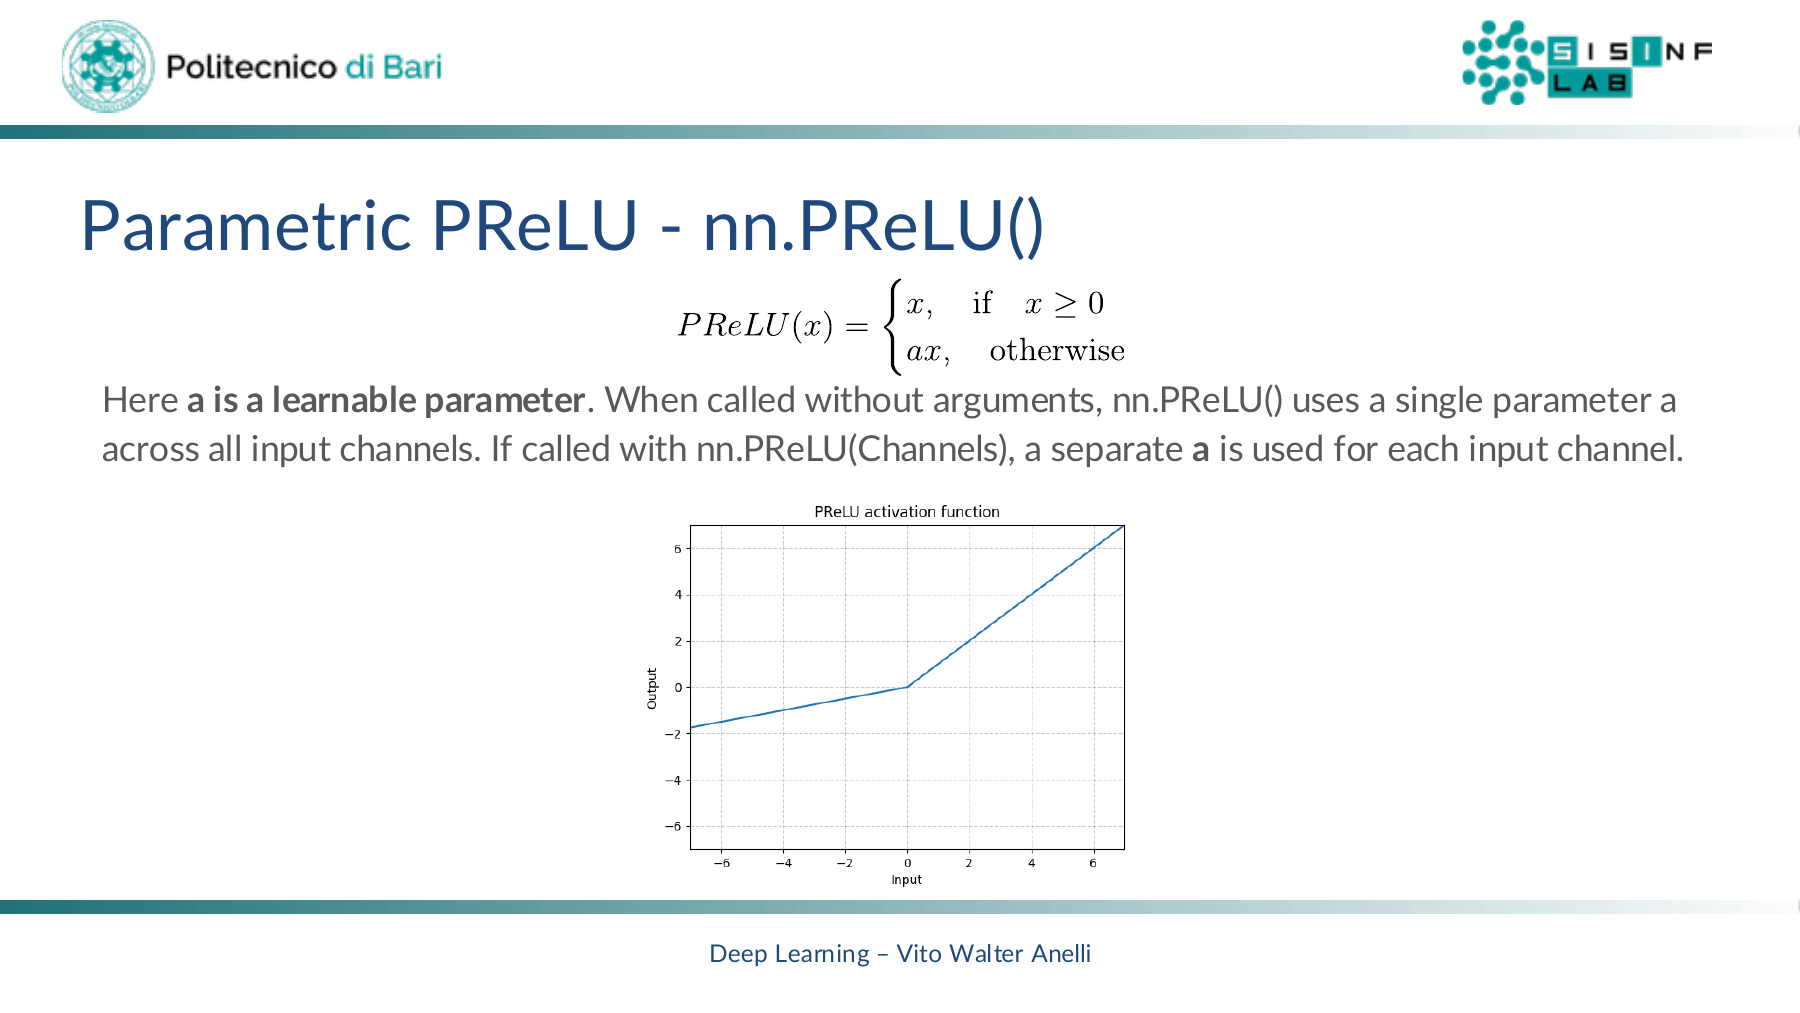
\includegraphics[width=0.72\linewidth]{figures/af03_prelu.png}
  \caption{Parametric ReLU (PReLU): il coefficiente $a$ è un \textbf{parametro
           apprendibile} con la retropropagazione. Chiamato senza argomenti,
           \texttt{nn.PReLU()} usa un unico parametro $a$ condiviso; chiamato
           con \texttt{nn.PReLU(C)}, usa un $a$ distinto per ognuno degli $C$
           canali in input.}
  \label{fig:prelu}
\end{figure}

La distinzione tra le tre varianti è riassumibile come segue:
\textbf{LReLU} usa un $a$ fisso, \textbf{PReLU} apprende $a$,
\textbf{RReLU} campiona $a$ casualmente durante il training.

\subsection{RReLU -- \texttt{nn.RReLU()}}
\label{subsec:rrelu}

\begin{equation}
  \operatorname{RReLU}(x) =
  \begin{cases}
    x,  & \text{se } x \geq 0 \\
    ax, & \text{altrimenti}
  \end{cases}
\end{equation}

\begin{figure}[H]
  \centering
  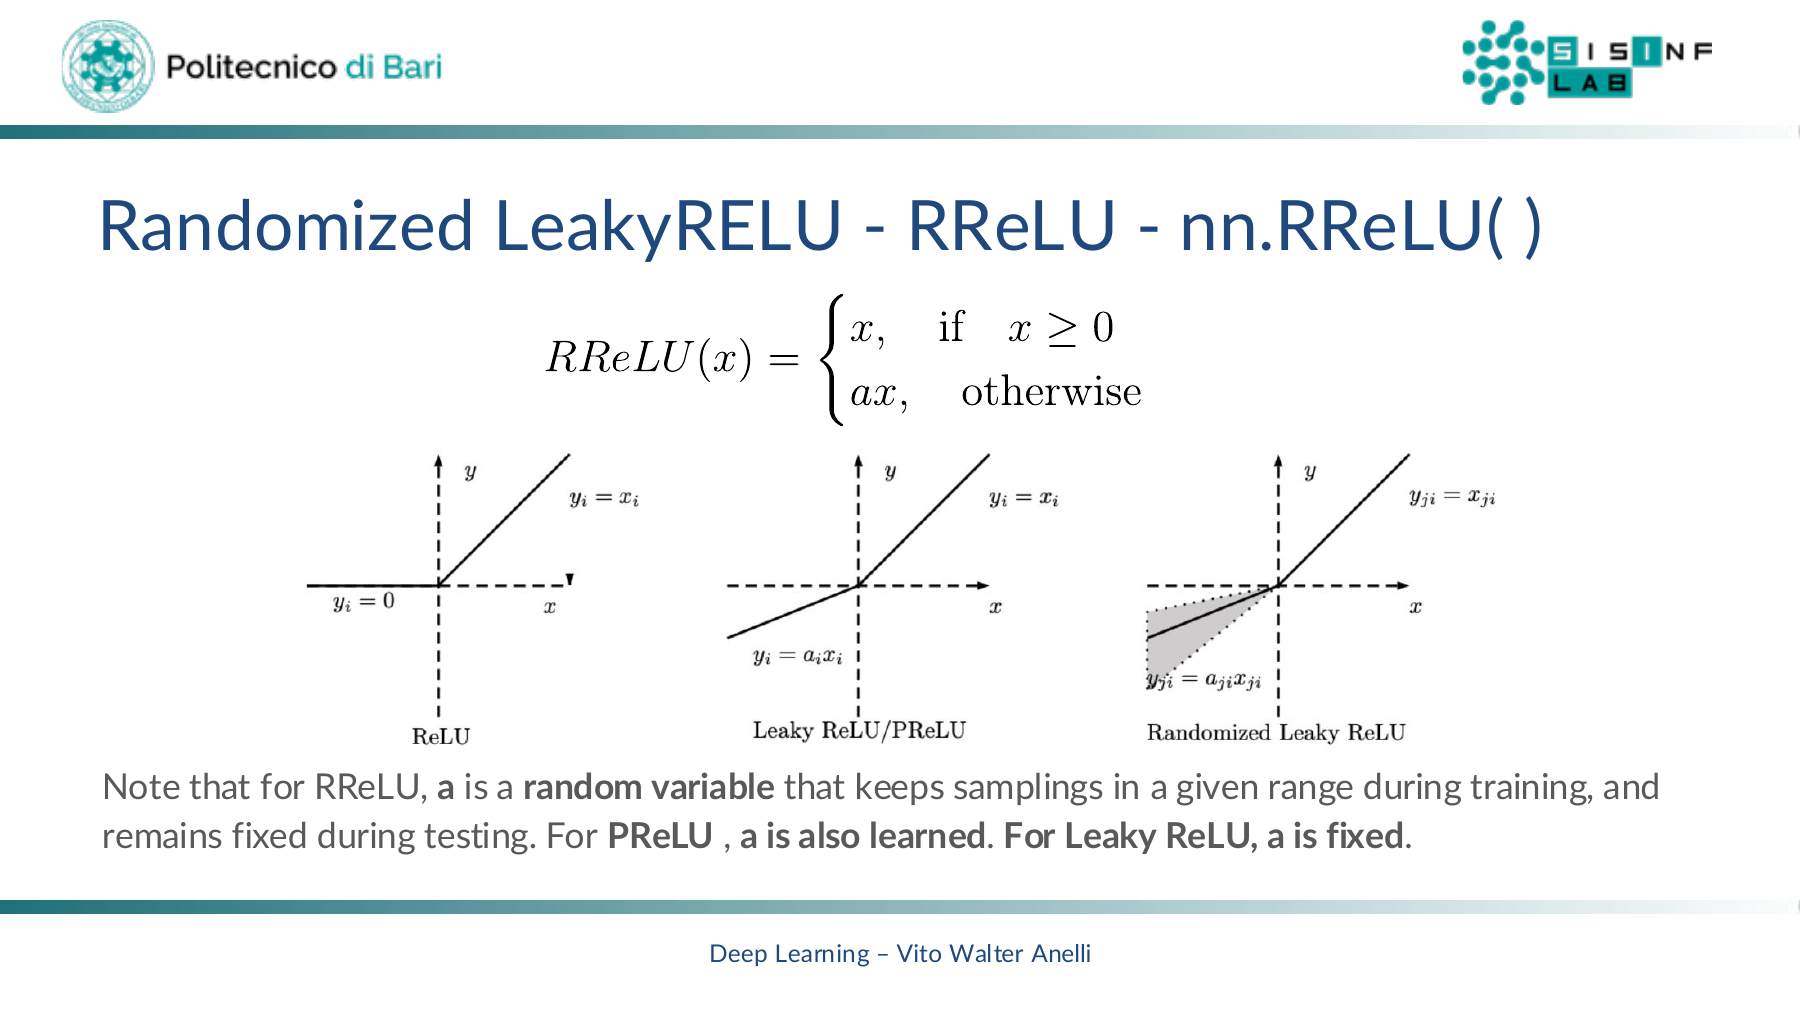
\includegraphics[width=0.85\linewidth]{figures/af03_rrelu.png}
  \caption{Confronto visivo tra ReLU, Leaky ReLU/PReLU e Randomized Leaky ReLU (RReLU).
           In RReLU, il parametro $a_{ji}$ è campionato uniformemente da un intervallo
           $[l,u]$ durante il training; al test viene usato il valor medio $(l+u)/2$.
           Questo effetto di randomizzazione funge da regolarizzazione implicita.}
  \label{fig:rrelu}
\end{figure}

\begin{figure}[H]
  \centering
  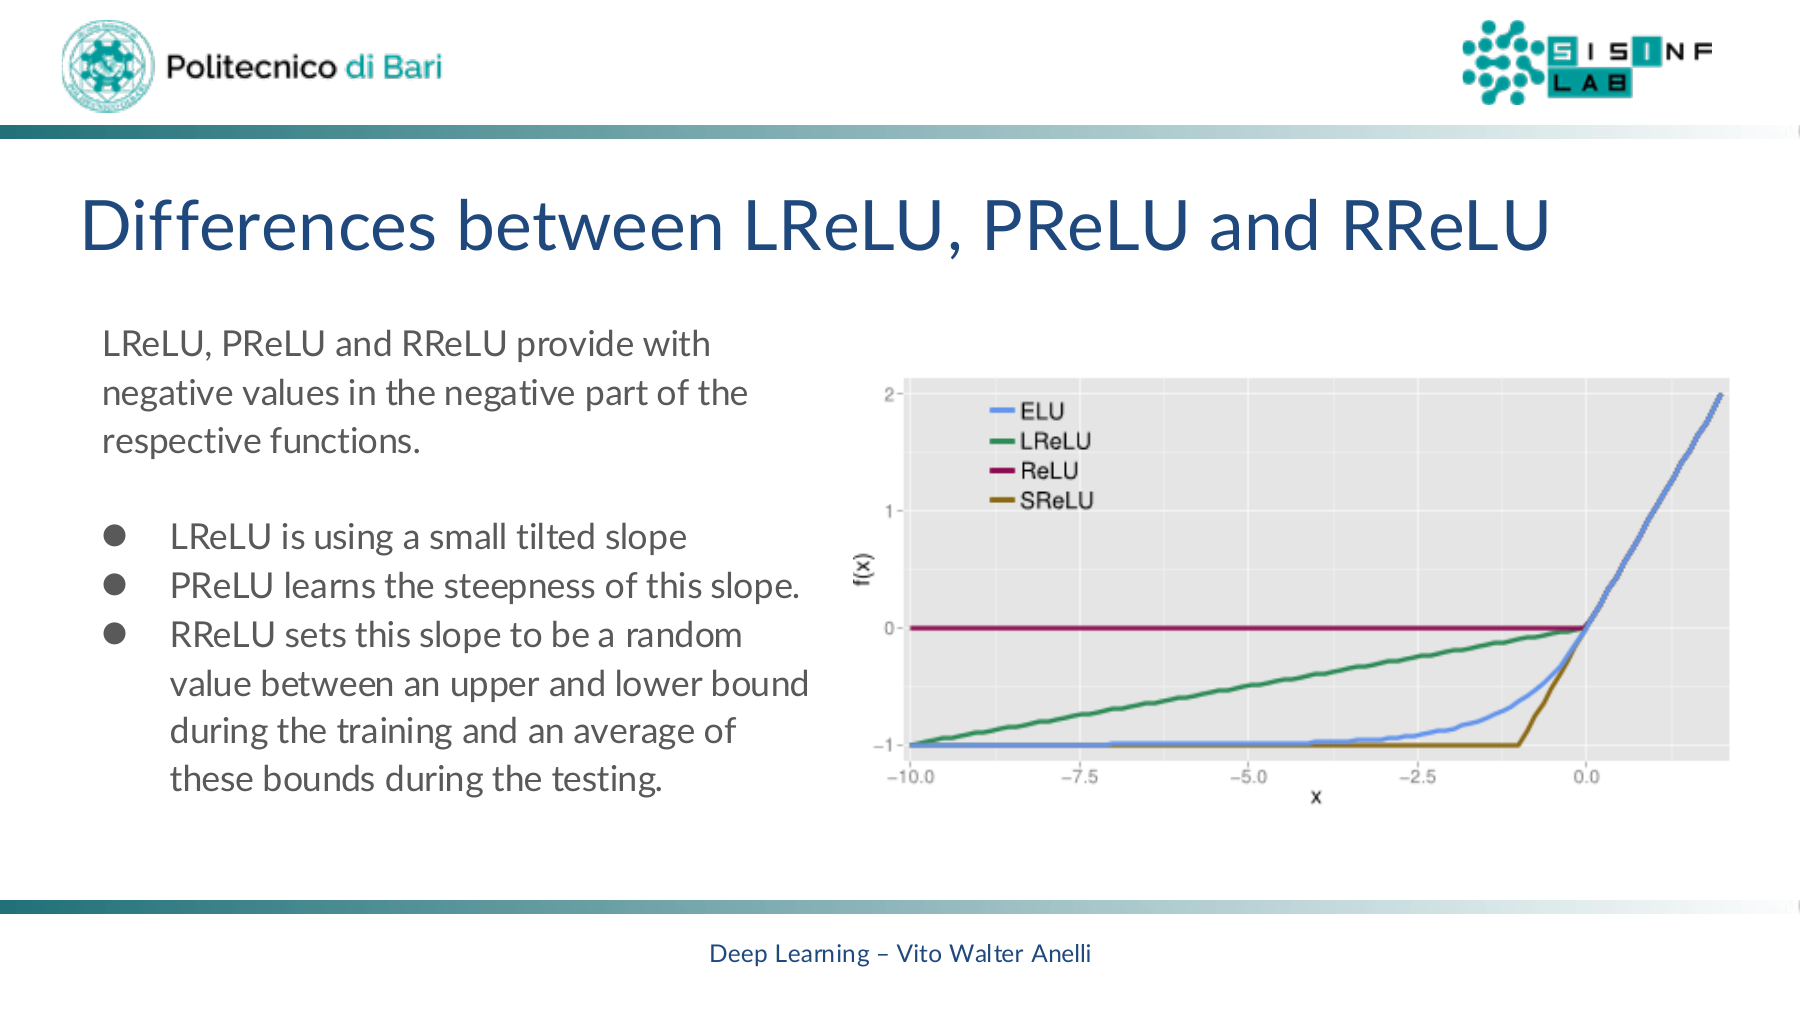
\includegraphics[width=0.80\linewidth]{figures/af03_lrelu_prelu_rrelu_diff.png}
  \caption{Differenze nella regione negativa tra ELU, LReLU, ReLU e SReLU.
           LReLU usa una pendenza fissa piccola; PReLU la apprende; RReLU
           la randomizza durante il training e la fissa alla media al test.}
  \label{fig:lrelu_prelu_rrelu_diff}
\end{figure}

\subsection{ReLU6 -- \texttt{nn.ReLU6()}}
\label{subsec:relu6}

\begin{equation}
  \operatorname{ReLU6}(x) = \min\!\bigl(\max(0, x),\, 6\bigr).
\end{equation}

\begin{figure}[H]
  \centering
  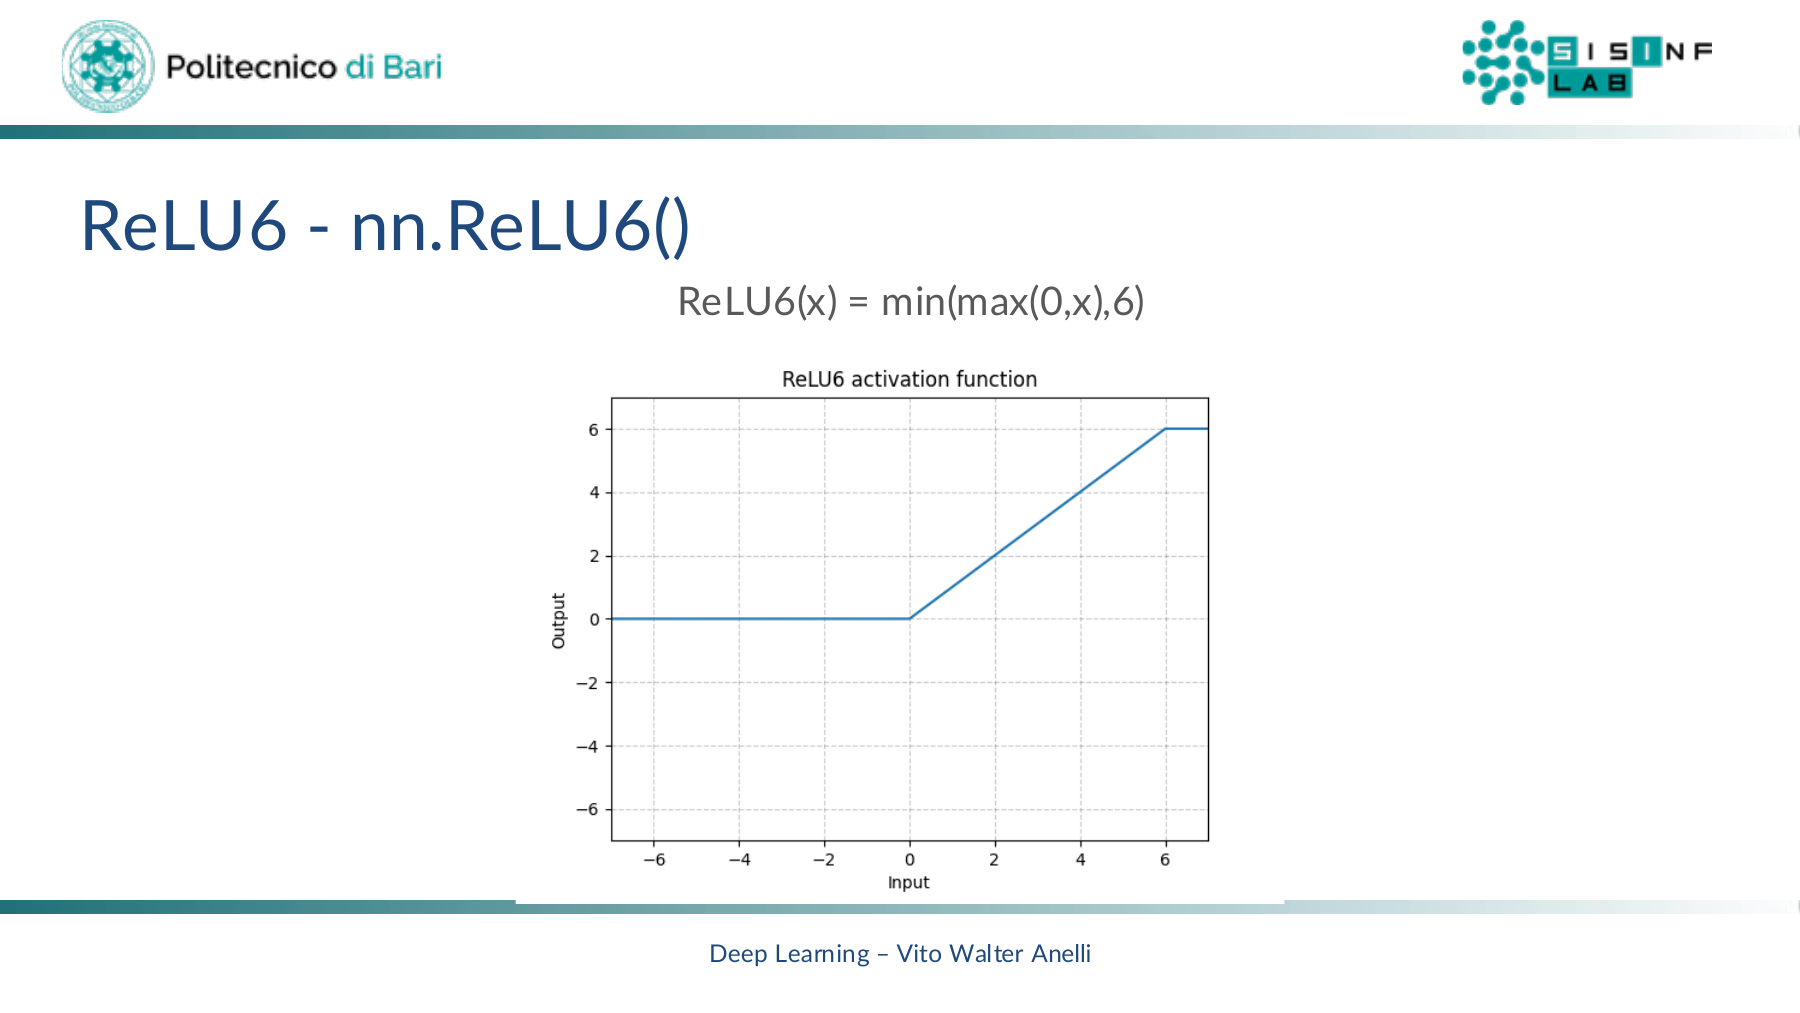
\includegraphics[width=0.72\linewidth]{figures/af03_relu6.png}
  \caption{ReLU6: ReLU con saturazione superiore a $6$. Progettata
           per ambienti a precisione ridotta (es.\ mobile/quantizzazione),
           previene attivazioni molto grandi che possono degradare la
           rappresentazione in virgola mobile a bassa precisione.}
  \label{fig:relu6}
\end{figure}

%------------------------------------------------------------
\section{Famiglia ELU}
\label{sec:elu-family}

\subsection{ELU -- \texttt{nn.ELU()}}
\label{subsec:elu}

La \textbf{Exponential Linear Unit} risolve sia il dead neuron problem sia il
problema delle medie non centrate in zero \citep{bishop2024}:

\begin{equation}
  \operatorname{ELU}(x) = \max(0,x) + \min\!\bigl(0,\, \alpha\cdot(\exp(x)-1)\bigr).
\end{equation}

\begin{figure}[H]
  \centering
  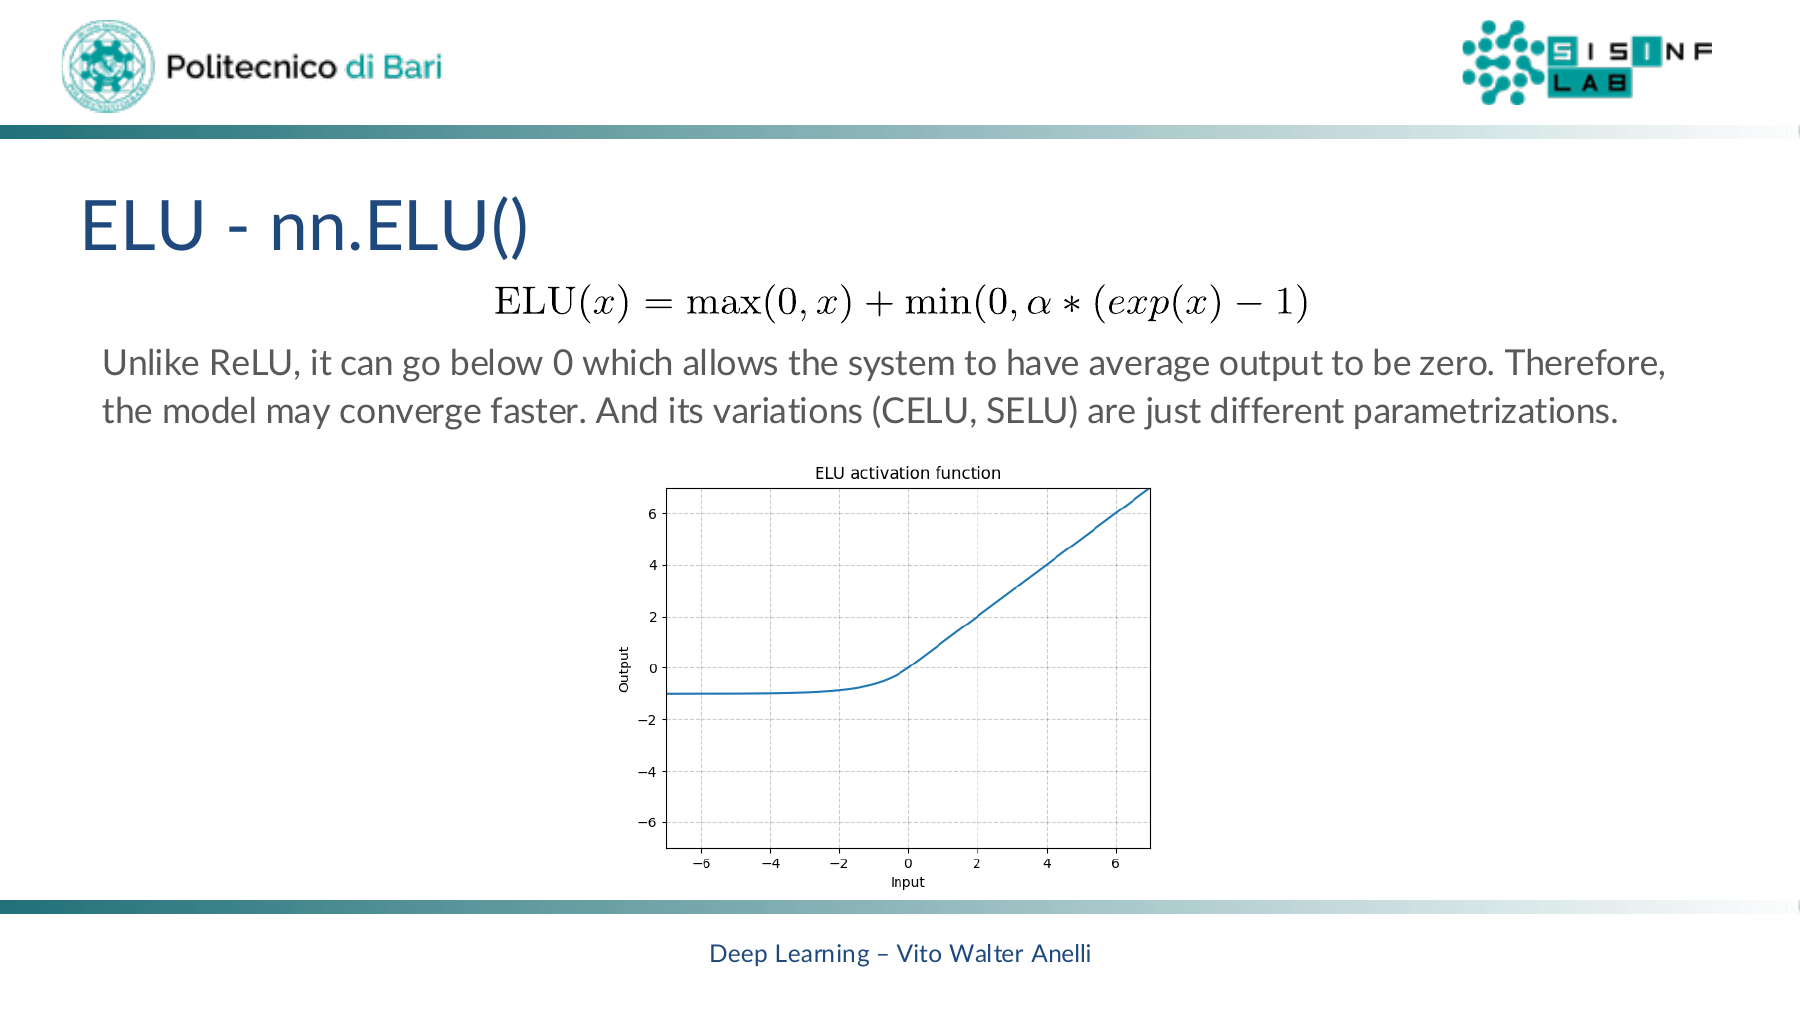
\includegraphics[width=0.72\linewidth]{figures/af03_elu.png}
  \caption{ELU: a differenza di ReLU, può produrre valori negativi,
           permettendo all'output medio del layer di essere vicino a zero.
           Questo centra le attivazioni e accelera la convergenza.
           Le varianti CELU e SELU sono reparametrizzazioni di ELU.}
  \label{fig:elu}
\end{figure}

Il valore $\alpha$ controlla il limite inferiore della regione negativa
(di default $\alpha = 1$). Avere output con media vicina a zero ha lo stesso
beneficio del \emph{Batch Normalization}: il gradiente non è sistematicamente
distorto, e la convergenza è più rapida.

\subsection{CELU -- \texttt{nn.CELU()}}
\label{subsec:celu}

\begin{equation}
  \operatorname{CELU}(x) = \max(0,x) + \min\!\left(0,\, \alpha \cdot
  \left(\exp\!\left(\frac{x}{\alpha}\right) - 1\right)\right).
\end{equation}

\begin{figure}[H]
  \centering
  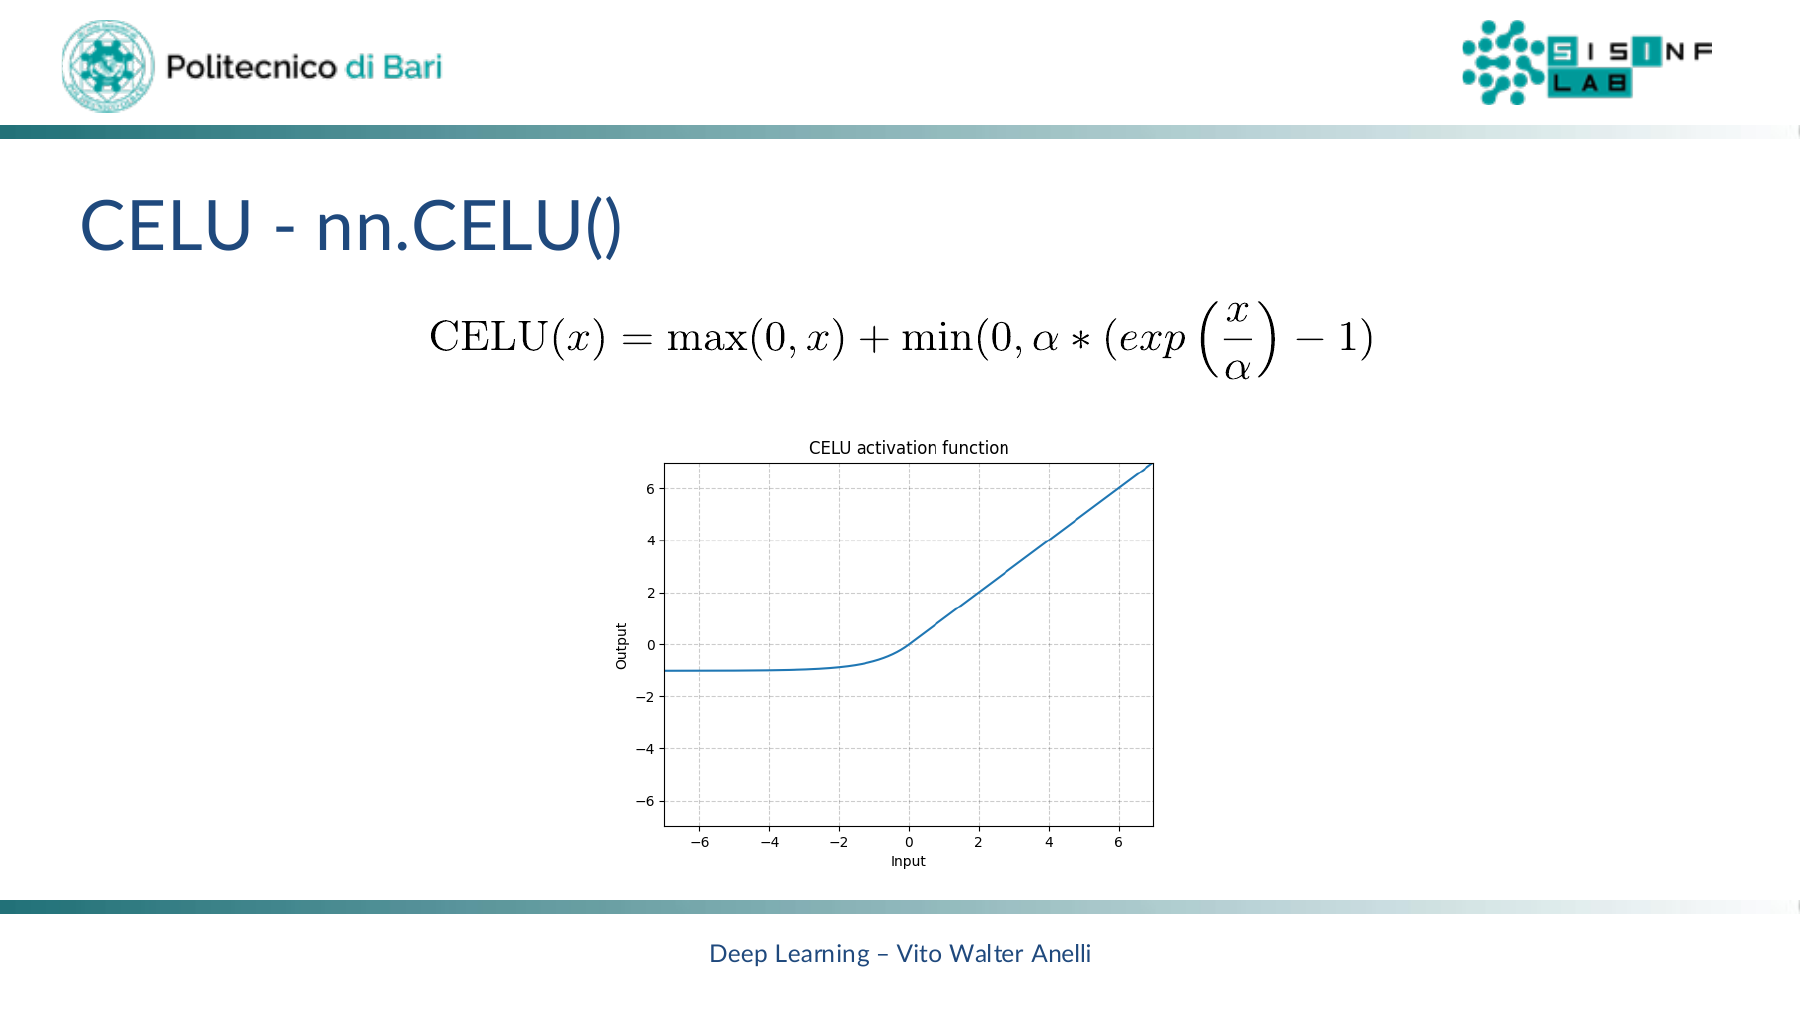
\includegraphics[width=0.72\linewidth]{figures/af03_celu.png}
  \caption{CELU (Continuously Differentiable ELU): reparametrizza ELU in modo
           da garantire la derivabilità continua in $x=0$ per qualsiasi valore
           di $\alpha$, migliorando la stabilità numerica del training.}
  \label{fig:celu}
\end{figure}

\subsection{SELU -- \texttt{nn.SELU()}}
\label{subsec:selu}

\begin{equation}
  \operatorname{SELU}(x) = \mathrm{scale} \cdot
  \bigl(\max(0,x) + \min\!\bigl(0,\,\alpha\cdot(\exp(x)-1)\bigr)\bigr),
\end{equation}
con $\mathrm{scale} \approx 1{,}0507$ e $\alpha \approx 1{,}6733$
(valori calcolati analiticamente da Klambauer et al., 2017).

\begin{figure}[H]
  \centering
  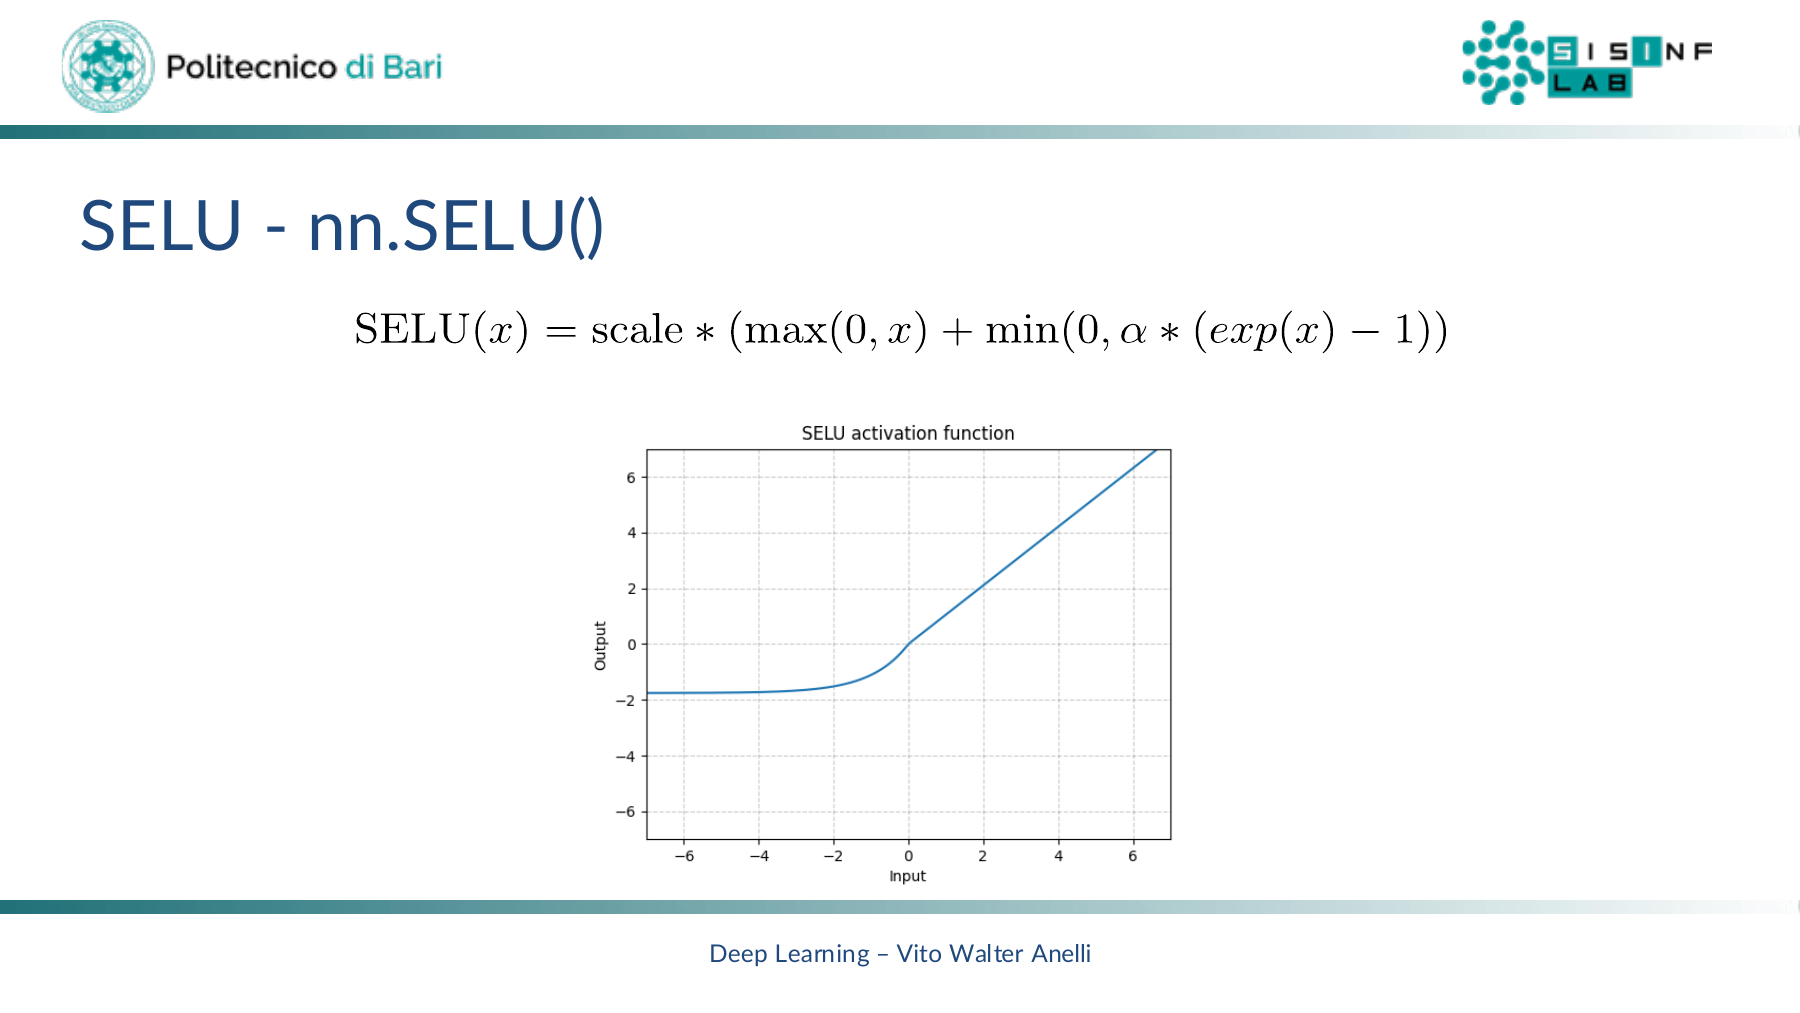
\includegraphics[width=0.72\linewidth]{figures/af03_selu.png}
  \caption{SELU (Scaled ELU): aggiunge un fattore di scala alla ELU.
           Con le costanti $\alpha$ e \emph{scale} opportune, la SELU garantisce
           \emph{self-normalizing} properties: attivazioni con media $0$ e
           varianza $1$ si propagano stabili attraverso layer arbitrariamente
           profondi, senza necessità di Batch Normalization.}
  \label{fig:selu}
\end{figure}

%------------------------------------------------------------
\section{Softplus e GELU}
\label{sec:softplus-gelu}

\subsection{Softplus -- \texttt{nn.Softplus()}}
\label{subsec:softplus}

\begin{equation}
  \operatorname{Softplus}(x) = \frac{1}{\beta} \cdot \log\!\bigl(1 + \exp(\beta x)\bigr).
\end{equation}

\begin{figure}[H]
  \centering
  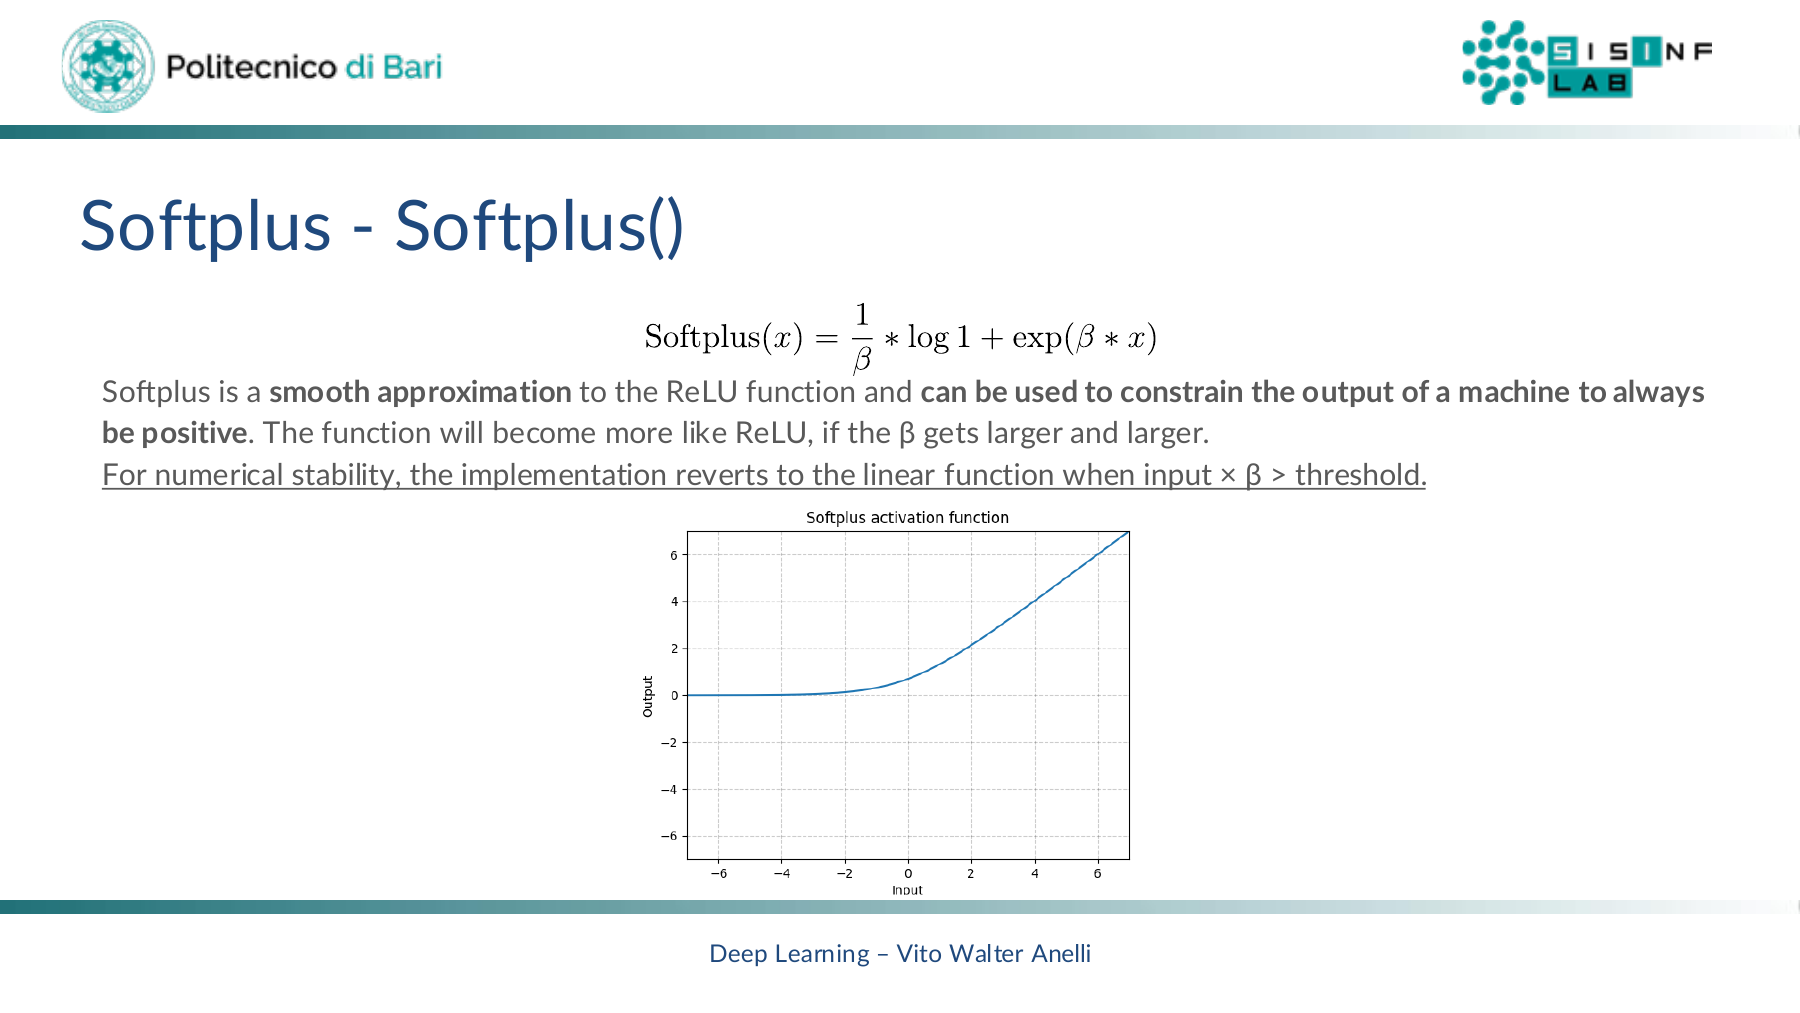
\includegraphics[width=0.72\linewidth]{figures/af03_softplus.png}
  \caption{Softplus: approssimazione \textbf{smooth} di ReLU, con derivata continua
           in tutto $\mathbb{R}$. All'aumentare di $\beta$ converge a ReLU.
           Può essere usata per \emph{vincolare l'output a essere sempre positivo}.
           Per stabilità numerica, l'implementazione torna alla funzione lineare
           quando $x \cdot \beta > \mathrm{threshold}$.}
  \label{fig:softplus}
\end{figure}

La Softplus è la primitiva della Sigmoid: $\frac{d}{dx}\operatorname{Softplus}(x) = \sigma(x)$,
il che ne chiarisce il ruolo teorico come ``versione continua'' di ReLU.

\subsection{GELU -- \texttt{nn.GELU()}}
\label{subsec:gelu}

\begin{equation}
  \operatorname{GELU}(x) = x \cdot \Phi(x),
\end{equation}
dove $\Phi(x)$ è la \emph{Cumulative Distribution Function} della distribuzione gaussiana standard.

\begin{figure}[H]
  \centering
  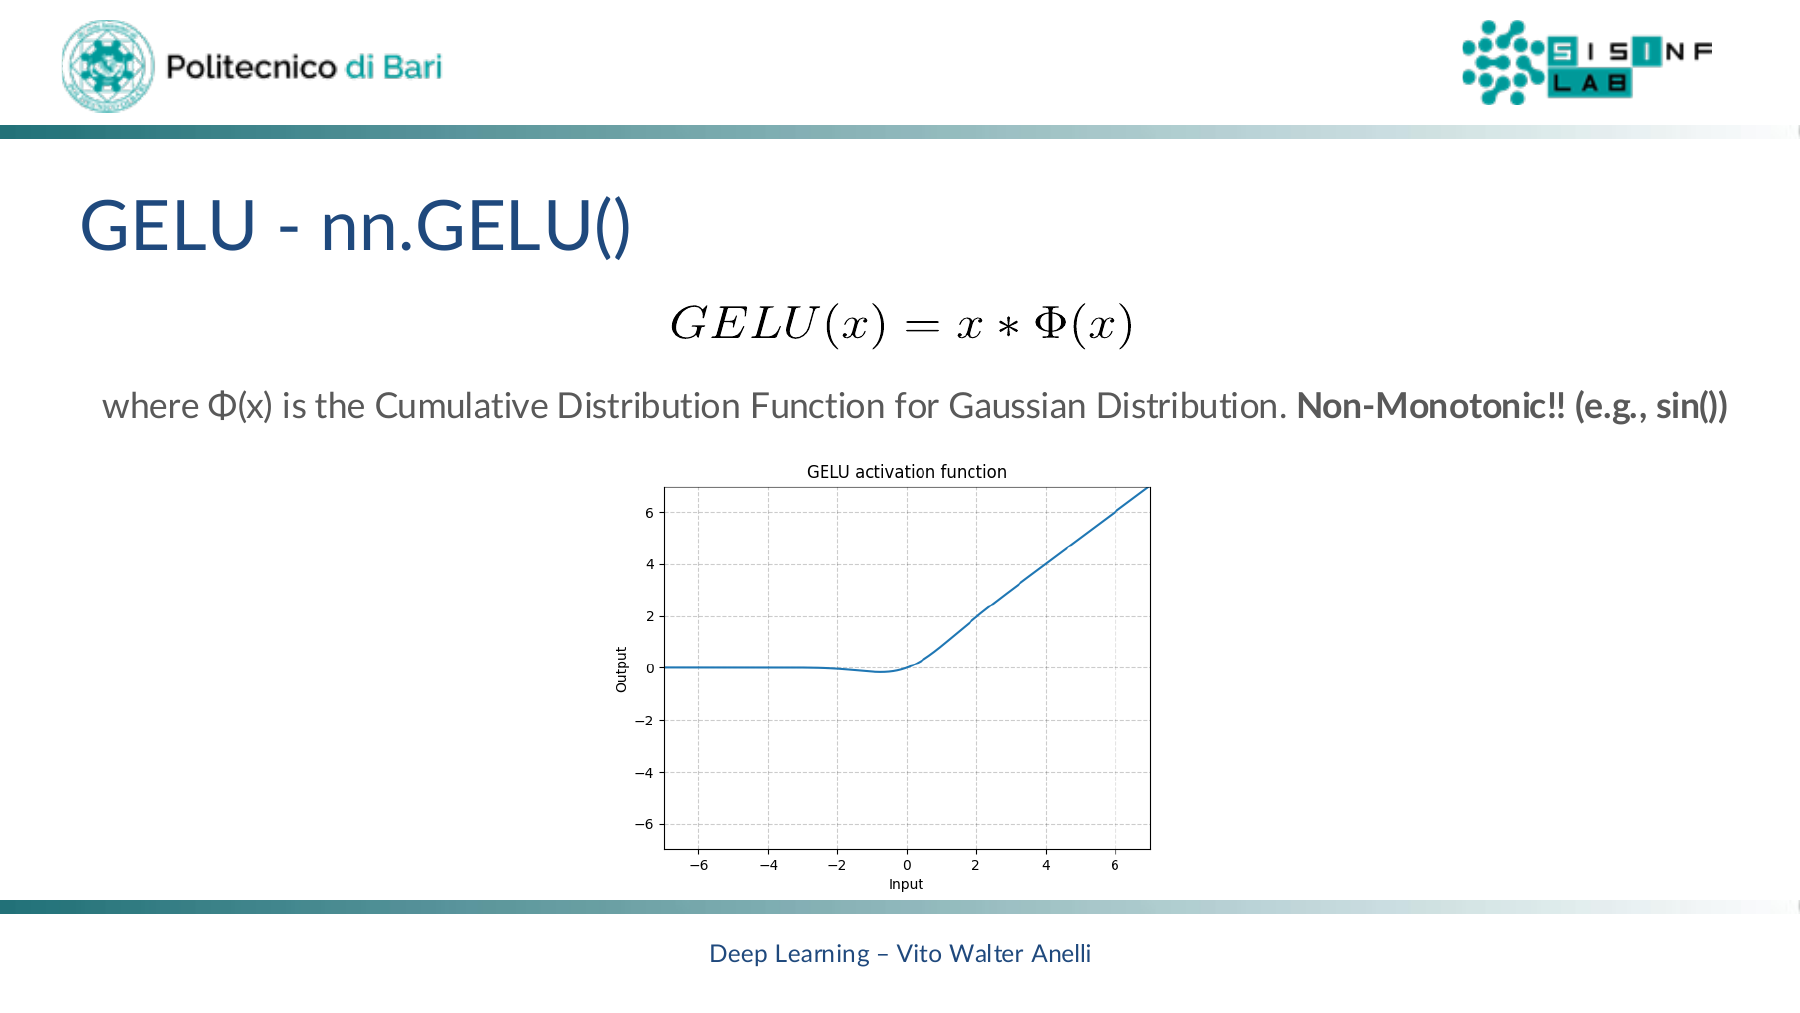
\includegraphics[width=0.72\linewidth]{figures/af03_gelu.png}
  \caption{GELU (Gaussian Error Linear Unit): funzione \textbf{non monotona},
           a differenza di ReLU e delle sue varianti. Nella regione $x < 0$
           l'output decresce, poi risale, imitando il comportamento del dropout
           stocastico. È la funzione di attivazione predefinita nei Transformer
           (BERT, GPT) per le sue proprietà di regolarizzazione implicita.}
  \label{fig:gelu}
\end{figure}

L'approssimazione pratica spesso utilizzata è:
\begin{equation}
  \operatorname{GELU}(x) \approx 0{,}5\, x
  \left(1 + \tanh\!\left[\sqrt{\frac{2}{\pi}}\bigl(x + 0{,}044715\, x^3\bigr)\right]\right).
\end{equation}

%------------------------------------------------------------
\section{Funzioni Saturanti}
\label{sec:saturating}

\subsection{Sigmoid -- \texttt{nn.Sigmoid()}}
\label{subsec:sigmoid}

\begin{equation}
  \operatorname{Sigmoid}(x) = \sigma(x) = \frac{1}{1 + \exp(-x)}.
\end{equation}

\begin{figure}[H]
  \centering
  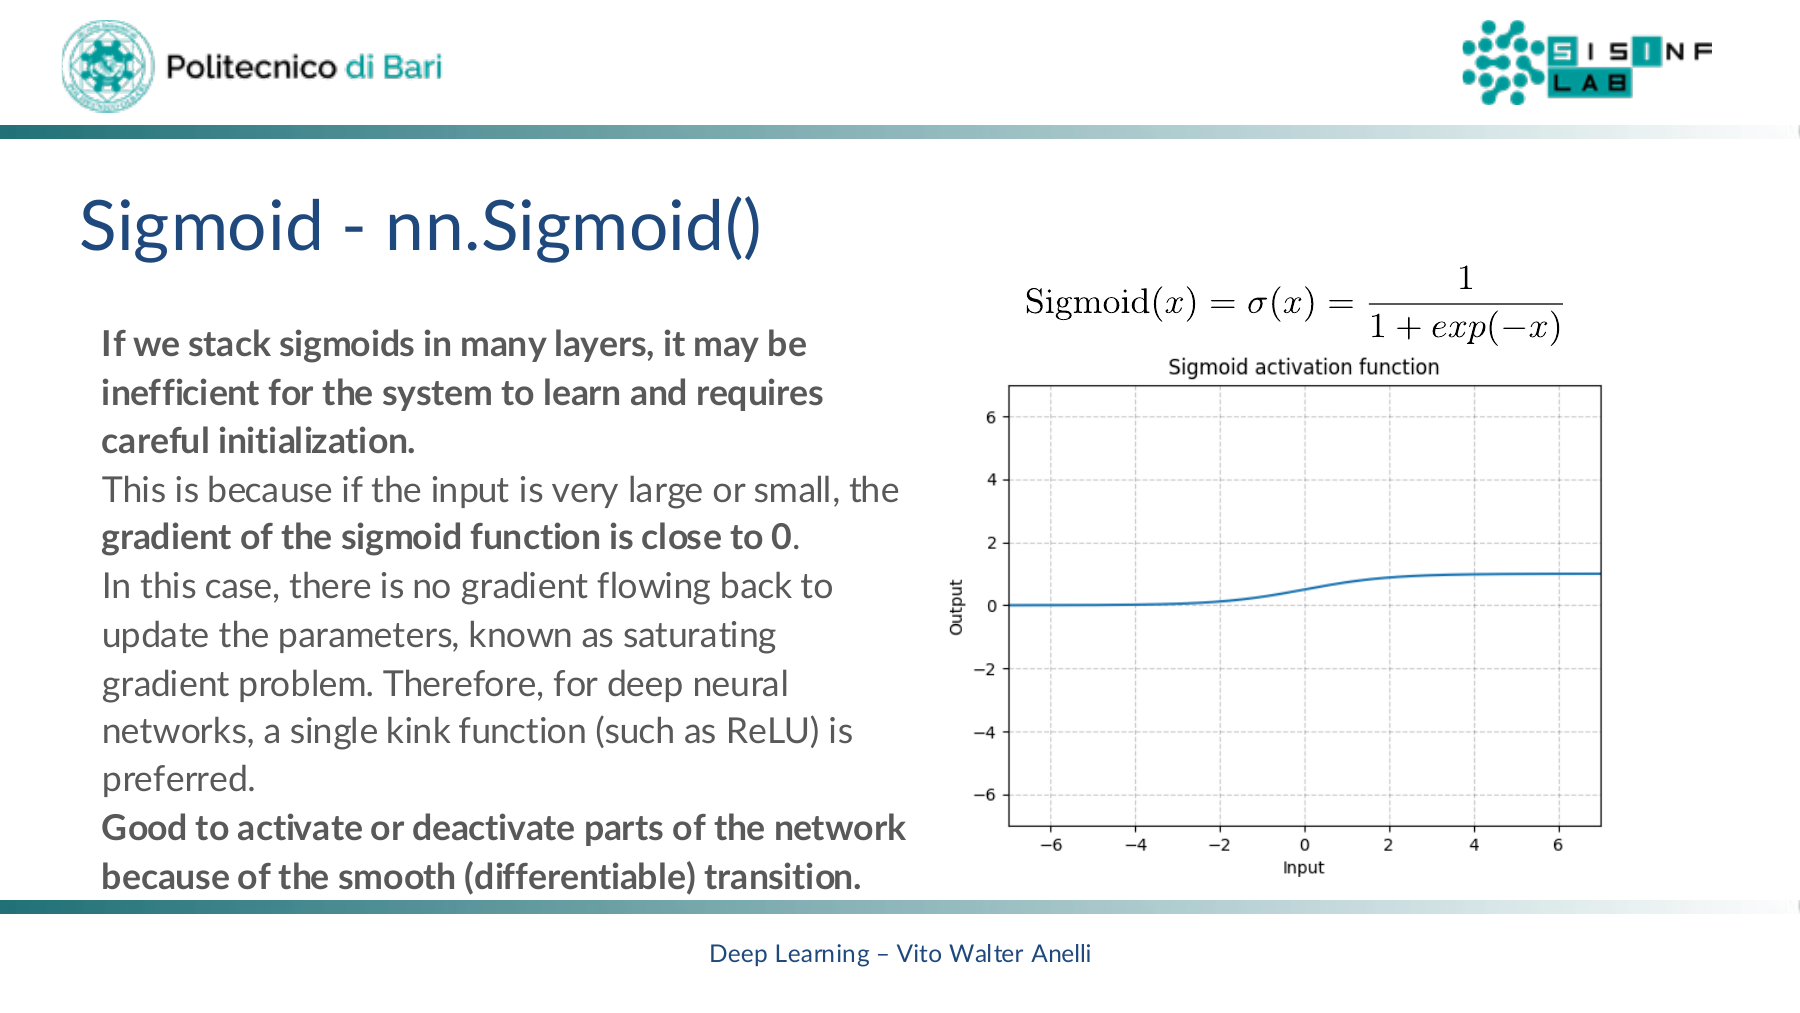
\includegraphics[width=0.85\linewidth]{figures/af03_sigmoid.png}
  \caption{Sigmoid: output in $(0,1)$, il che la rende ideale come gate
           (LSTM, GRU) o per output probabilistici di classificatori binari.
           Impilare molti layer sigmoid causa il vanishing gradient: il gradiente
           della sigmoid è prossimo a zero per $|x| \gg 0$, bloccando la
           retropropagazione. Per reti profonde si preferisce ReLU.}
  \label{fig:sigmoid}
\end{figure}

\paragraph{Connessione con Softmax.}
Come mostrato nelle slide (Sez.~\ref{sec:softmax}), la Sigmoid è un caso
speciale della Softmax a due classi: posto $x_2 = 0$,
\begin{equation}
  z_1 = \frac{e^{x_1}}{e^{x_1}+e^{x_2}}
      = \frac{e^{x_1}}{e^{x_1}+1}
      = \frac{1}{1+e^{-x_1}} = \sigma(x_1).
\end{equation}

\subsection{Tanh -- \texttt{nn.Tanh()}}
\label{subsec:tanh}

\begin{equation}
  \operatorname{Tanh}(x) = \tanh(x) = \frac{\exp(x) - \exp(-x)}{\exp(x) + \exp(-x)}.
\end{equation}

\begin{figure}[H]
  \centering
  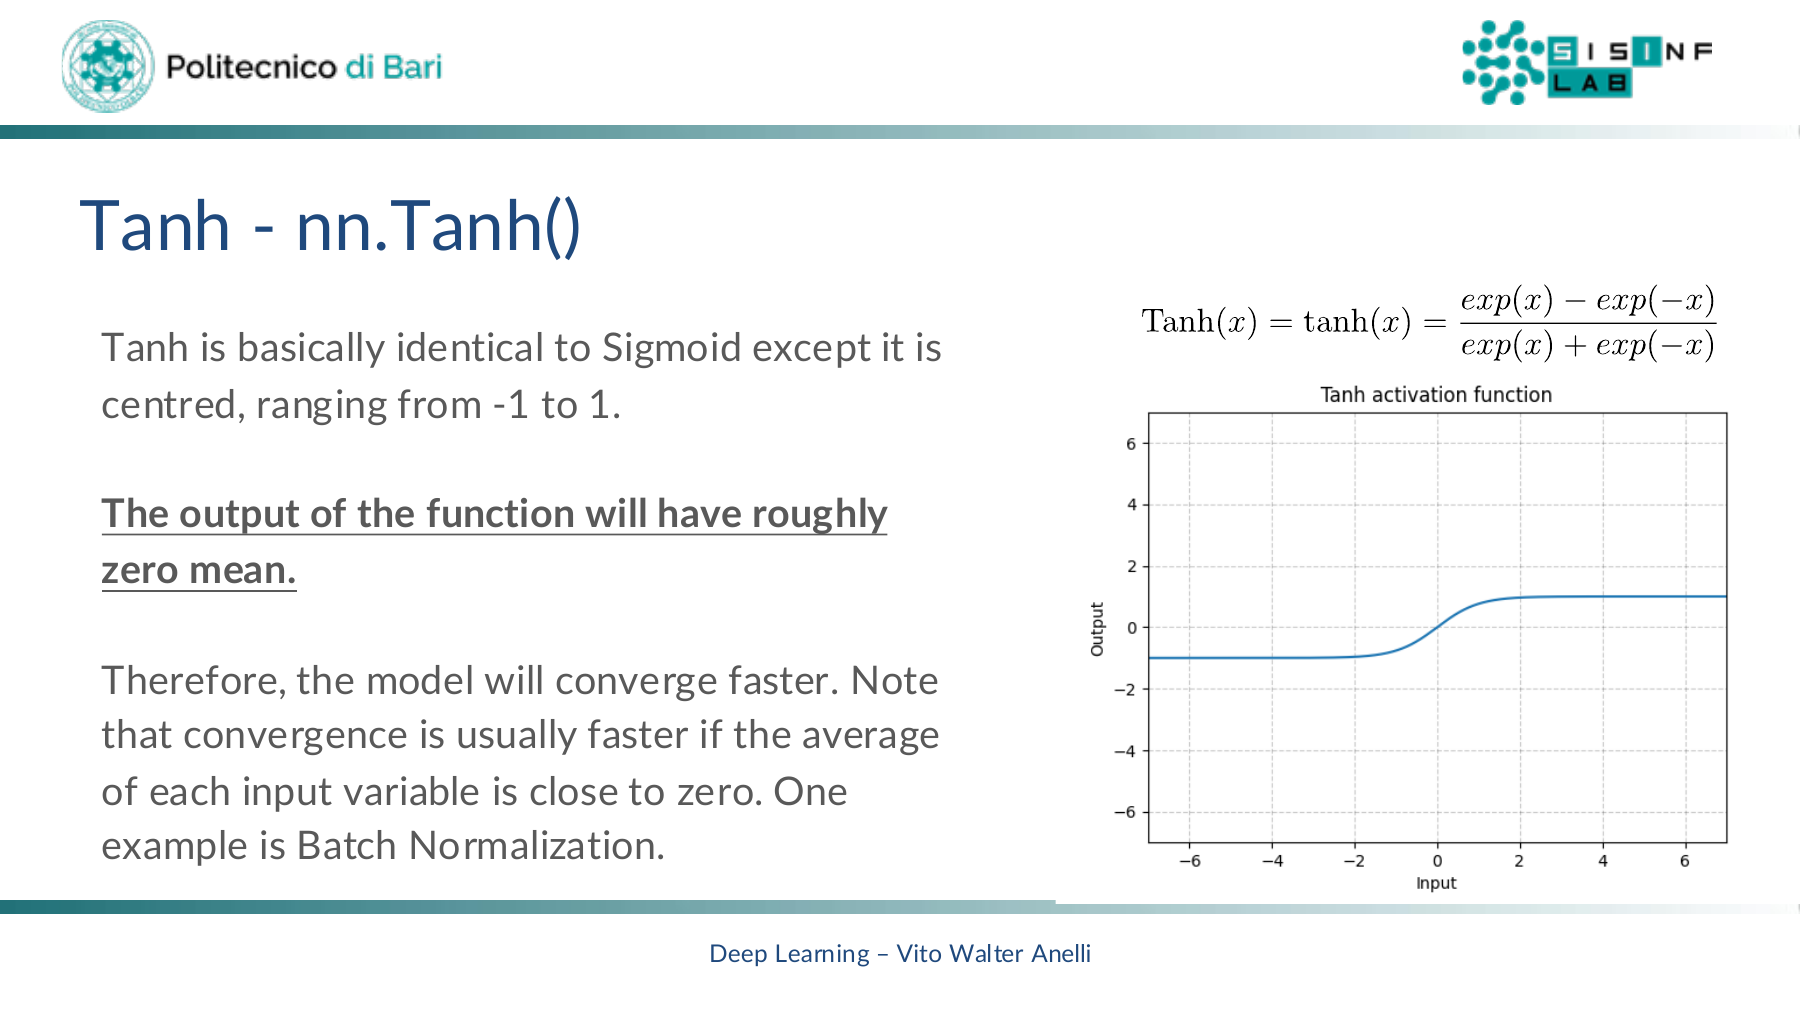
\includegraphics[width=0.85\linewidth]{figures/af03_tanh.png}
  \caption{Tanh: versione centrata della Sigmoid con output in $(-1, 1)$.
           L'output ha media approssimativamente zero, accelerando la convergenza
           rispetto a Sigmoid (nota fondamentale: la convergenza è più rapida
           quando la media degli input è vicina a zero, come avviene nel
           Batch Normalization). Soffre comunque del vanishing gradient.}
  \label{fig:tanh}
\end{figure}

\paragraph{Relazione con Sigmoid.}
$\tanh(x) = 2\sigma(2x) - 1$: Tanh è semplicemente una Sigmoid riscalata e
traslata. Preferire Tanh a Sigmoid nei layer nascosti perché l'output centrato
evita bias sistematici nel gradiente \citep{bishop2024}.

\subsection{Hardtanh -- \texttt{nn.Hardtanh()}}
\label{subsec:hardtanh}

\begin{equation}
  \operatorname{Hardtanh}(x) =
  \begin{cases}
    1,  & \text{se } x > 1 \\
    -1, & \text{se } x < -1 \\
    x,  & \text{altrimenti}
  \end{cases}
\end{equation}

\begin{figure}[H]
  \centering
  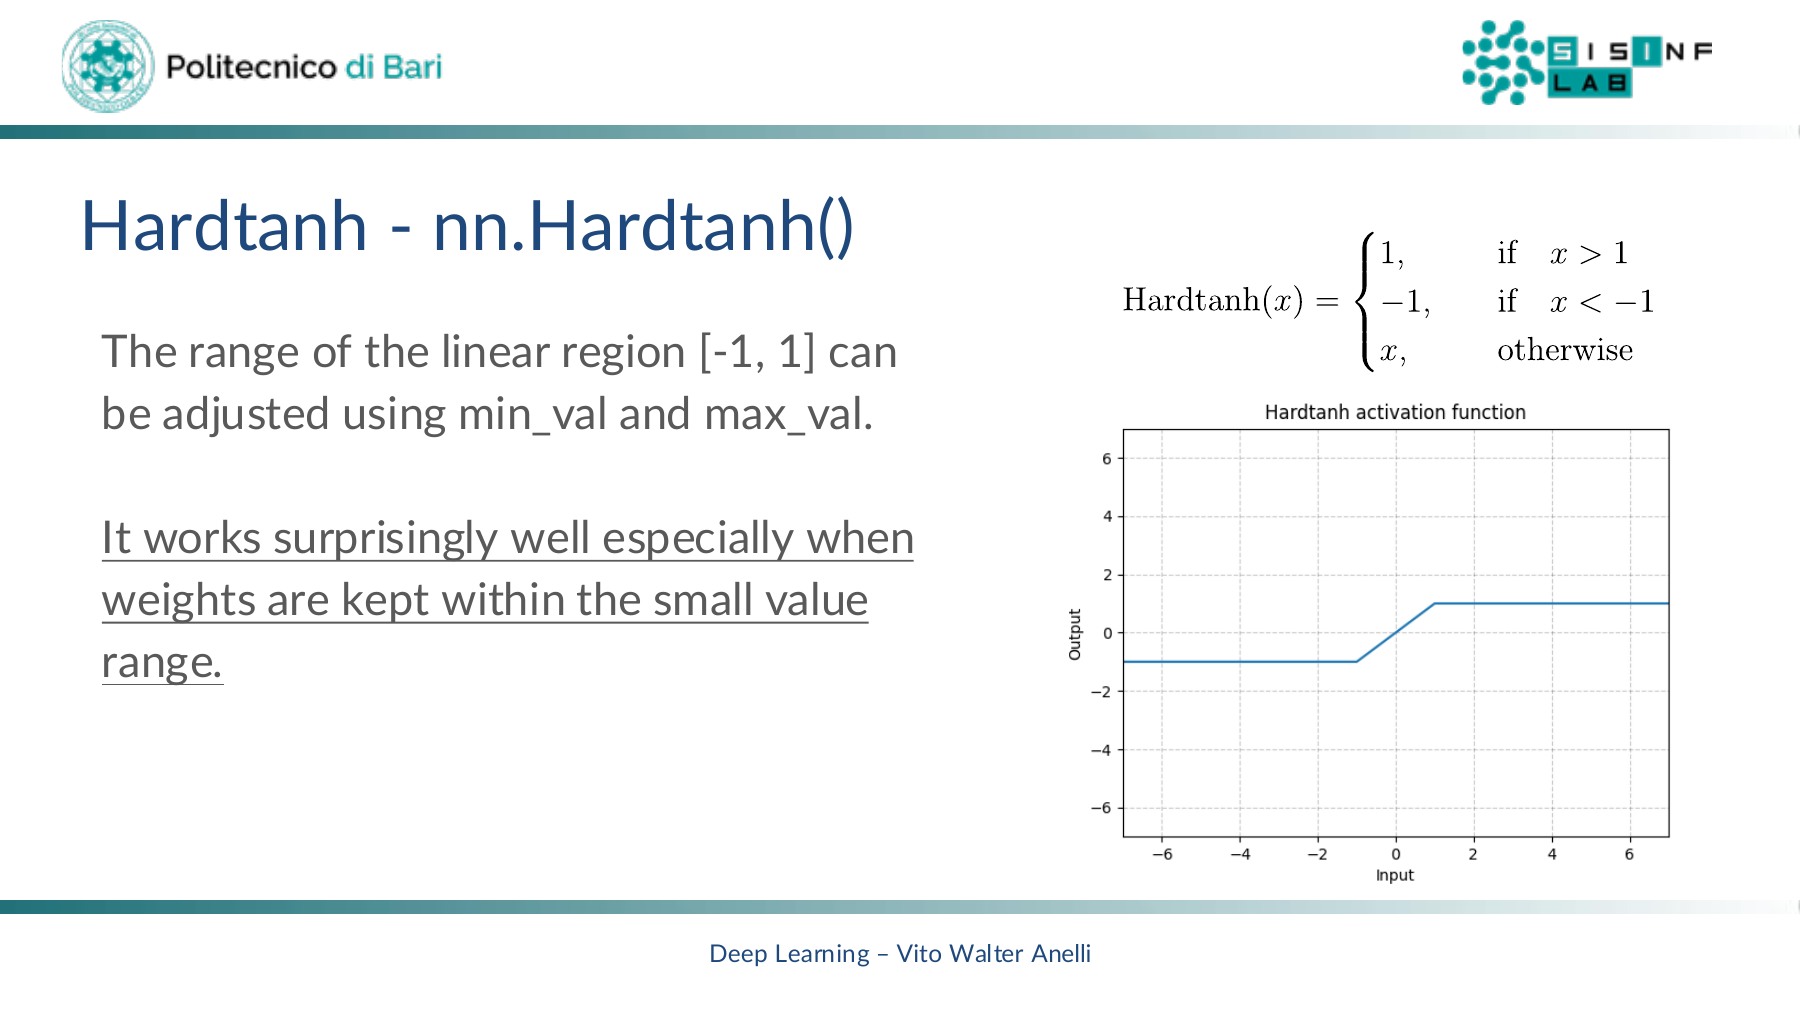
\includegraphics[width=0.85\linewidth]{figures/af03_hardtanh.png}
  \caption{Hardtanh: approssimazione lineare a tratti di Tanh.
           I valori di saturazione $[-1, 1]$ sono regolabili tramite
           \texttt{min\_val} e \texttt{max\_val}. Funziona sorprendentemente
           bene quando i pesi rimangono in un range di valori piccoli, ed è
           computazionalmente più leggera di Tanh.}
  \label{fig:hardtanh}
\end{figure}

\subsection{Softsign -- \texttt{nn.Softsign()}}
\label{subsec:softsign}

\begin{equation}
  \operatorname{SoftSign}(x) = \frac{x}{1 + |x|}.
\end{equation}

\begin{figure}[H]
  \centering
  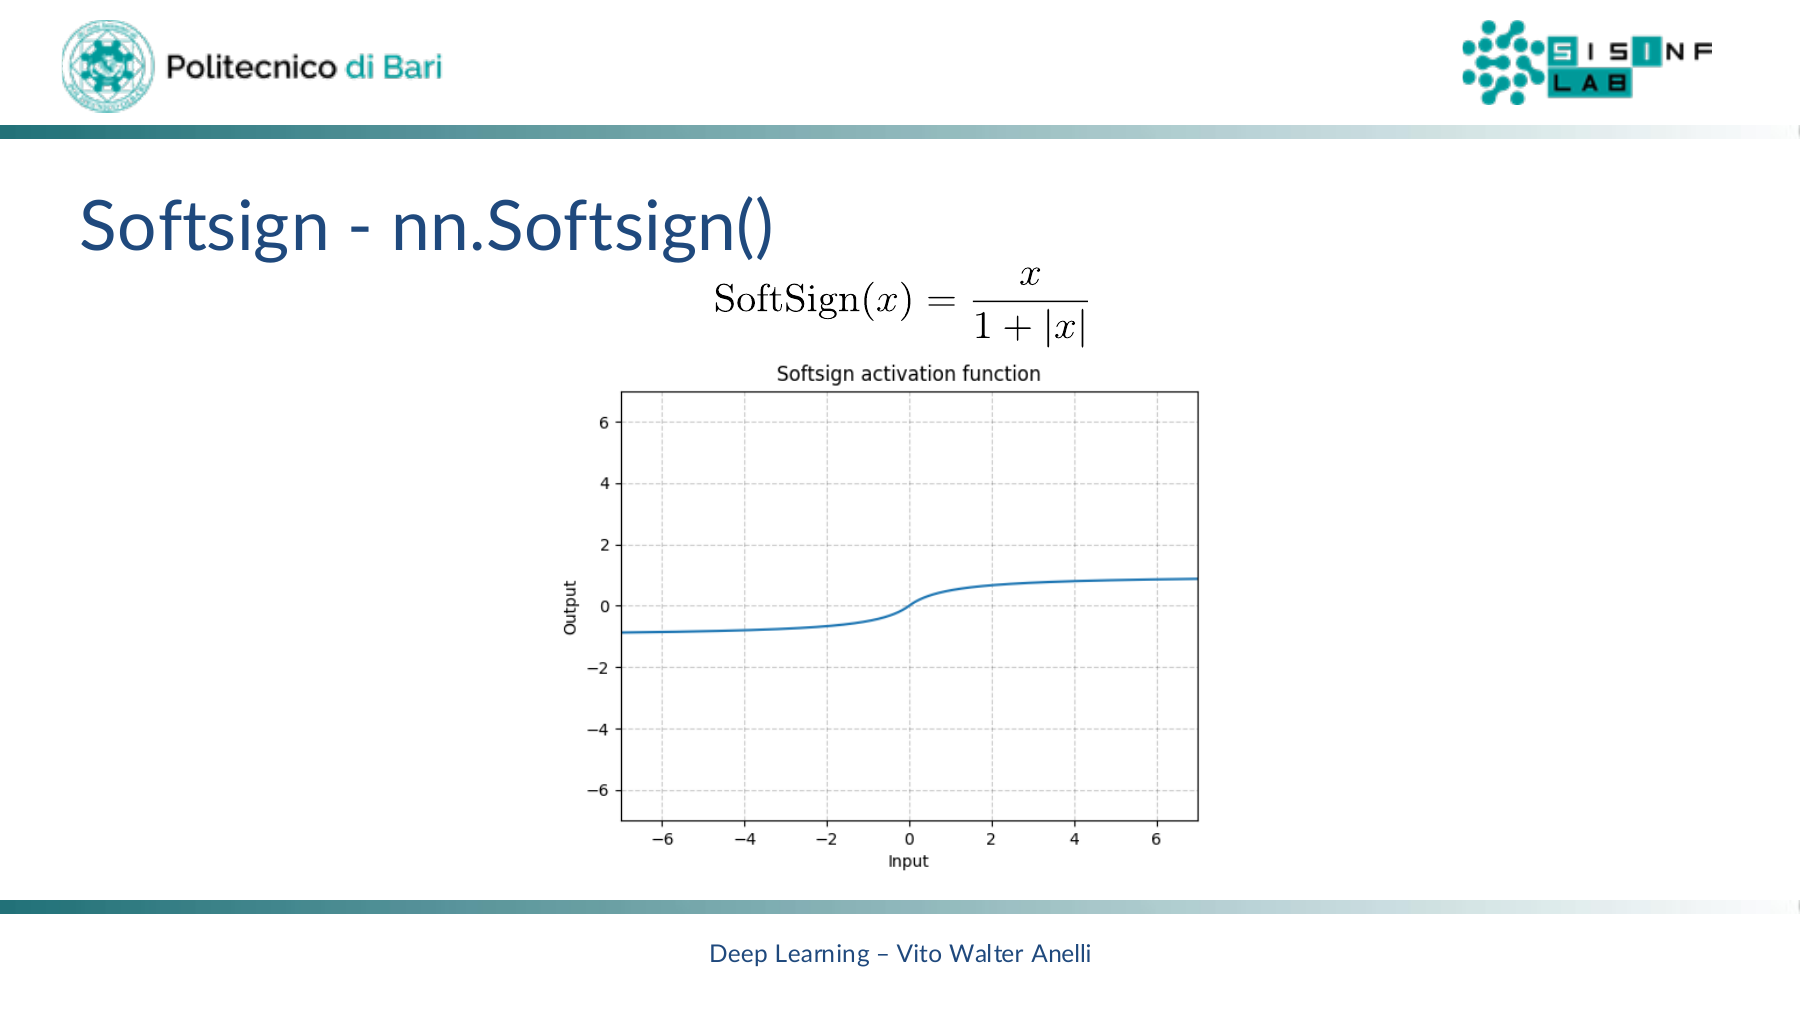
\includegraphics[width=0.72\linewidth]{figures/af03_softsign.png}
  \caption{Softsign: alternativa a Tanh con saturazione più lenta
           (decadimento polinomiale anziché esponenziale). Le code più
           pesanti implicano gradienti meno soggetti al vanishing problem
           rispetto a Tanh, ma l'output rimane in $(-1,1)$.}
  \label{fig:softsign}
\end{figure}

%------------------------------------------------------------
\section{Funzioni Shrink e Threshold}
\label{sec:shrink-threshold}

\subsection{Threshold -- \texttt{nn.Threshold()}}
\label{subsec:threshold}

\begin{equation}
  \operatorname{threshold}(x) =
  \begin{cases}
    x, & \text{se } x > \mathrm{threshold} \\
    v, & \text{altrimenti}
  \end{cases}
\end{equation}

\begin{figure}[H]
  \centering
  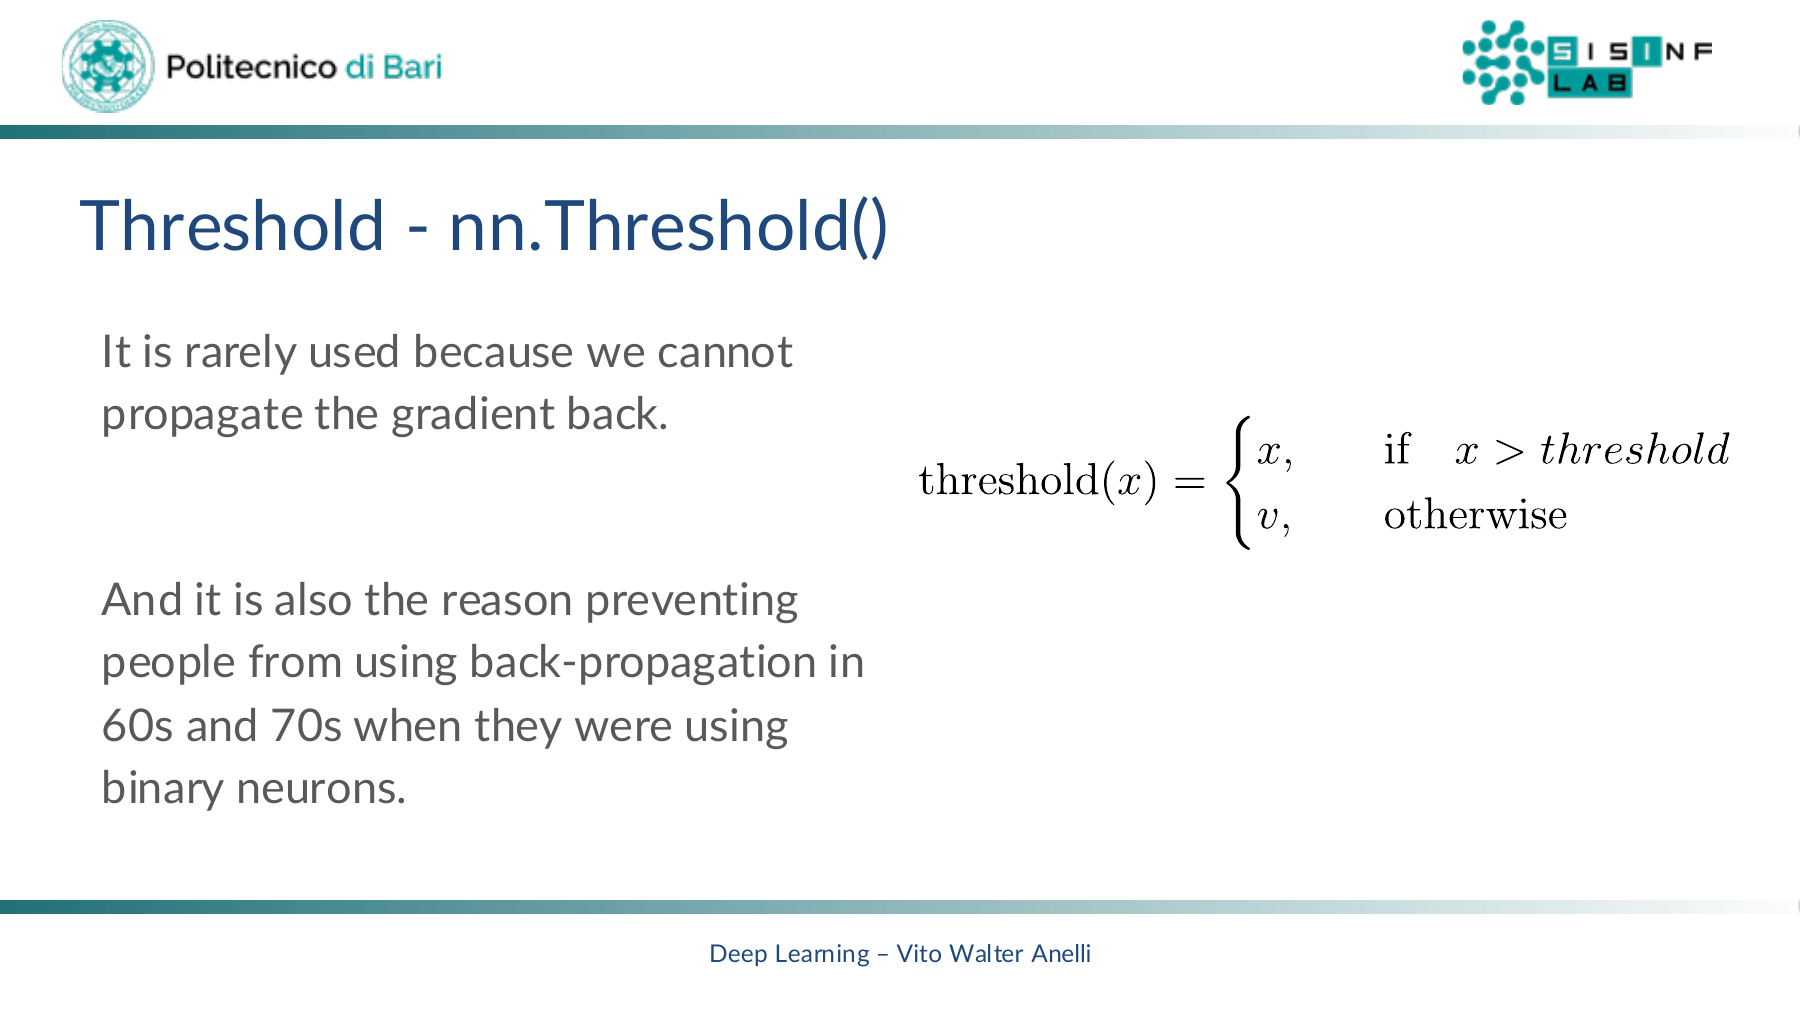
\includegraphics[width=0.72\linewidth]{figures/af03_threshold.png}
  \caption{Threshold (neurone binario): il gradiente è zero nella regione
           subthreshold, rendendo impossibile la retropropagazione per quei neuroni.
           È la ragione storica per cui la backpropagation non venne adottata
           negli anni '60--'70, quando si usavano neuroni binari.
           Attualmente non è utilizzata in reti moderne.}
  \label{fig:threshold}
\end{figure}

\subsection{Tanhshrink -- \texttt{nn.Tanhshrink()}}
\label{subsec:tanhshrink}

\begin{equation}
  \operatorname{Tanhshrink}(x) = x - \tanh(x).
\end{equation}

\begin{figure}[H]
  \centering
  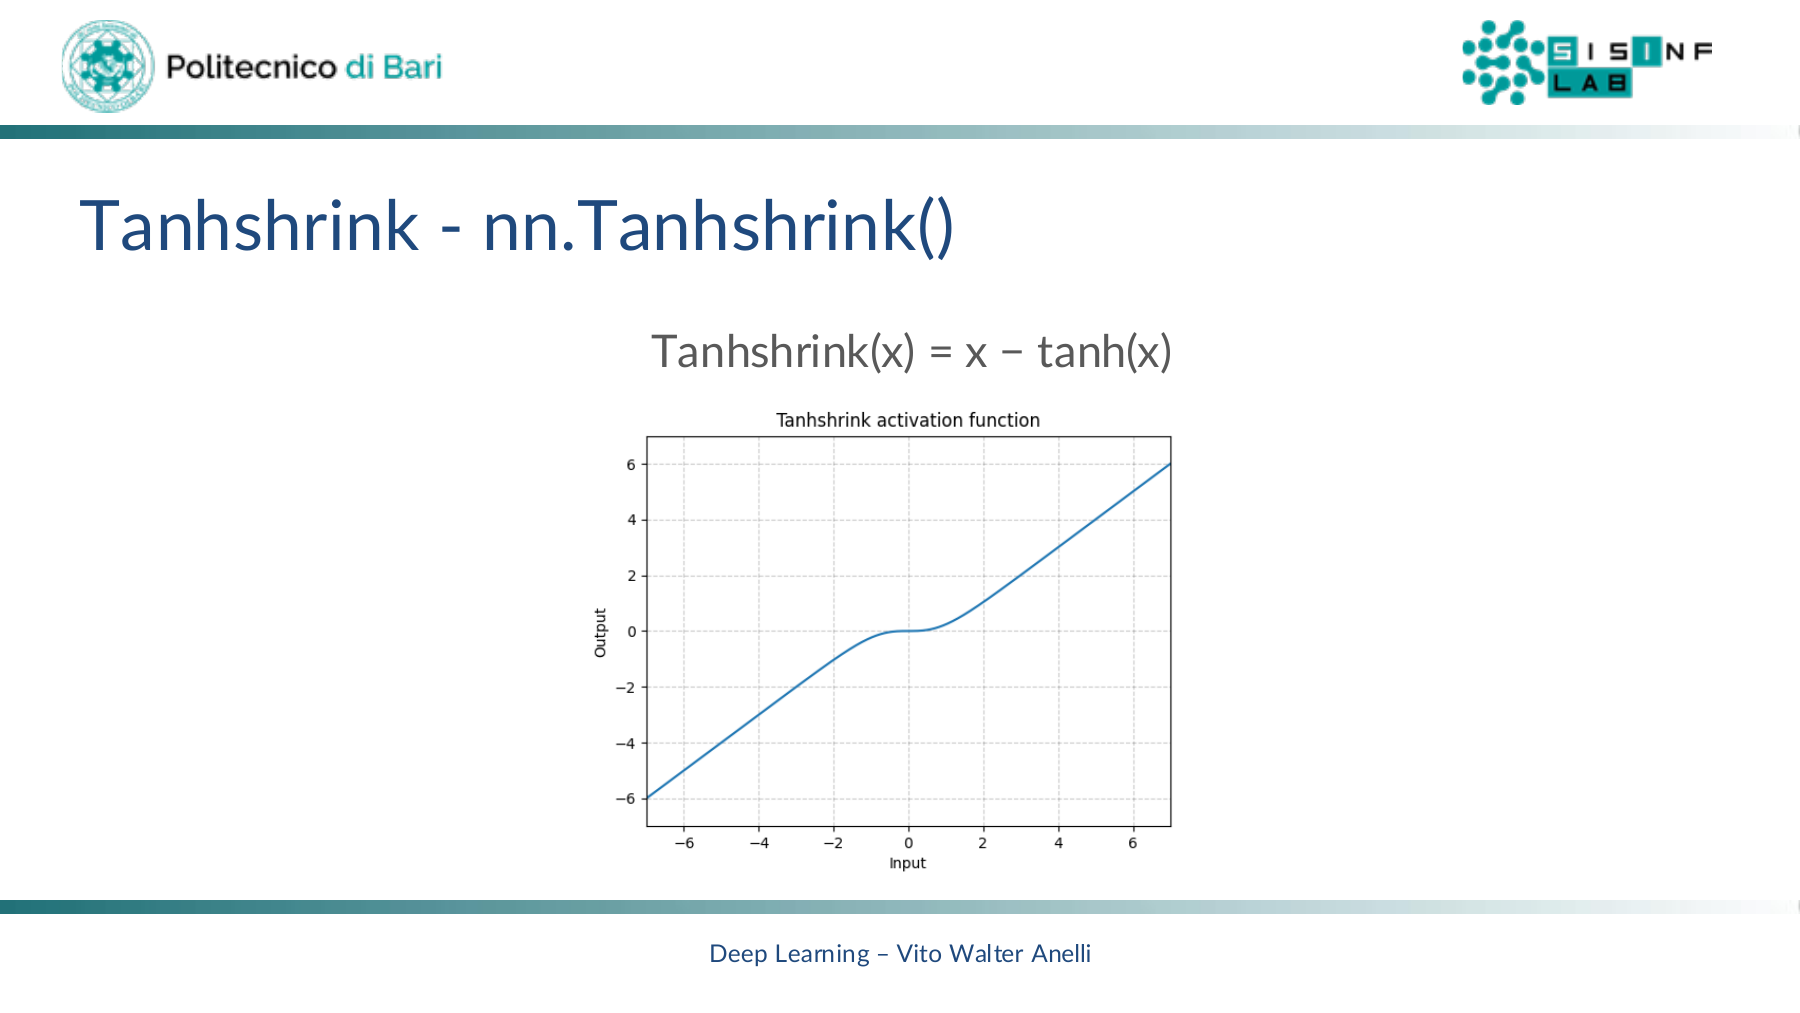
\includegraphics[width=0.72\linewidth]{figures/af03_tanhshrink.png}
  \caption{Tanhshrink: sottrae $\tanh(x)$ dall'input, producendo una funzione
           quasi lineare (con una lieve curvatura centrale). Usata in contesti
           di sparse coding per promuovere rappresentazioni sparse.}
  \label{fig:tanhshrink}
\end{figure}

\subsection{Softshrink -- \texttt{nn.Softshrink()}}
\label{subsec:softshrink}

\begin{equation}
  \operatorname{Softshrinkage}(x) =
  \begin{cases}
    x - \lambda, & \text{se } x > \lambda \\
    x + \lambda, & \text{se } x < -\lambda \\
    0,           & \text{altrimenti}
  \end{cases}
\end{equation}

\begin{figure}[H]
  \centering
  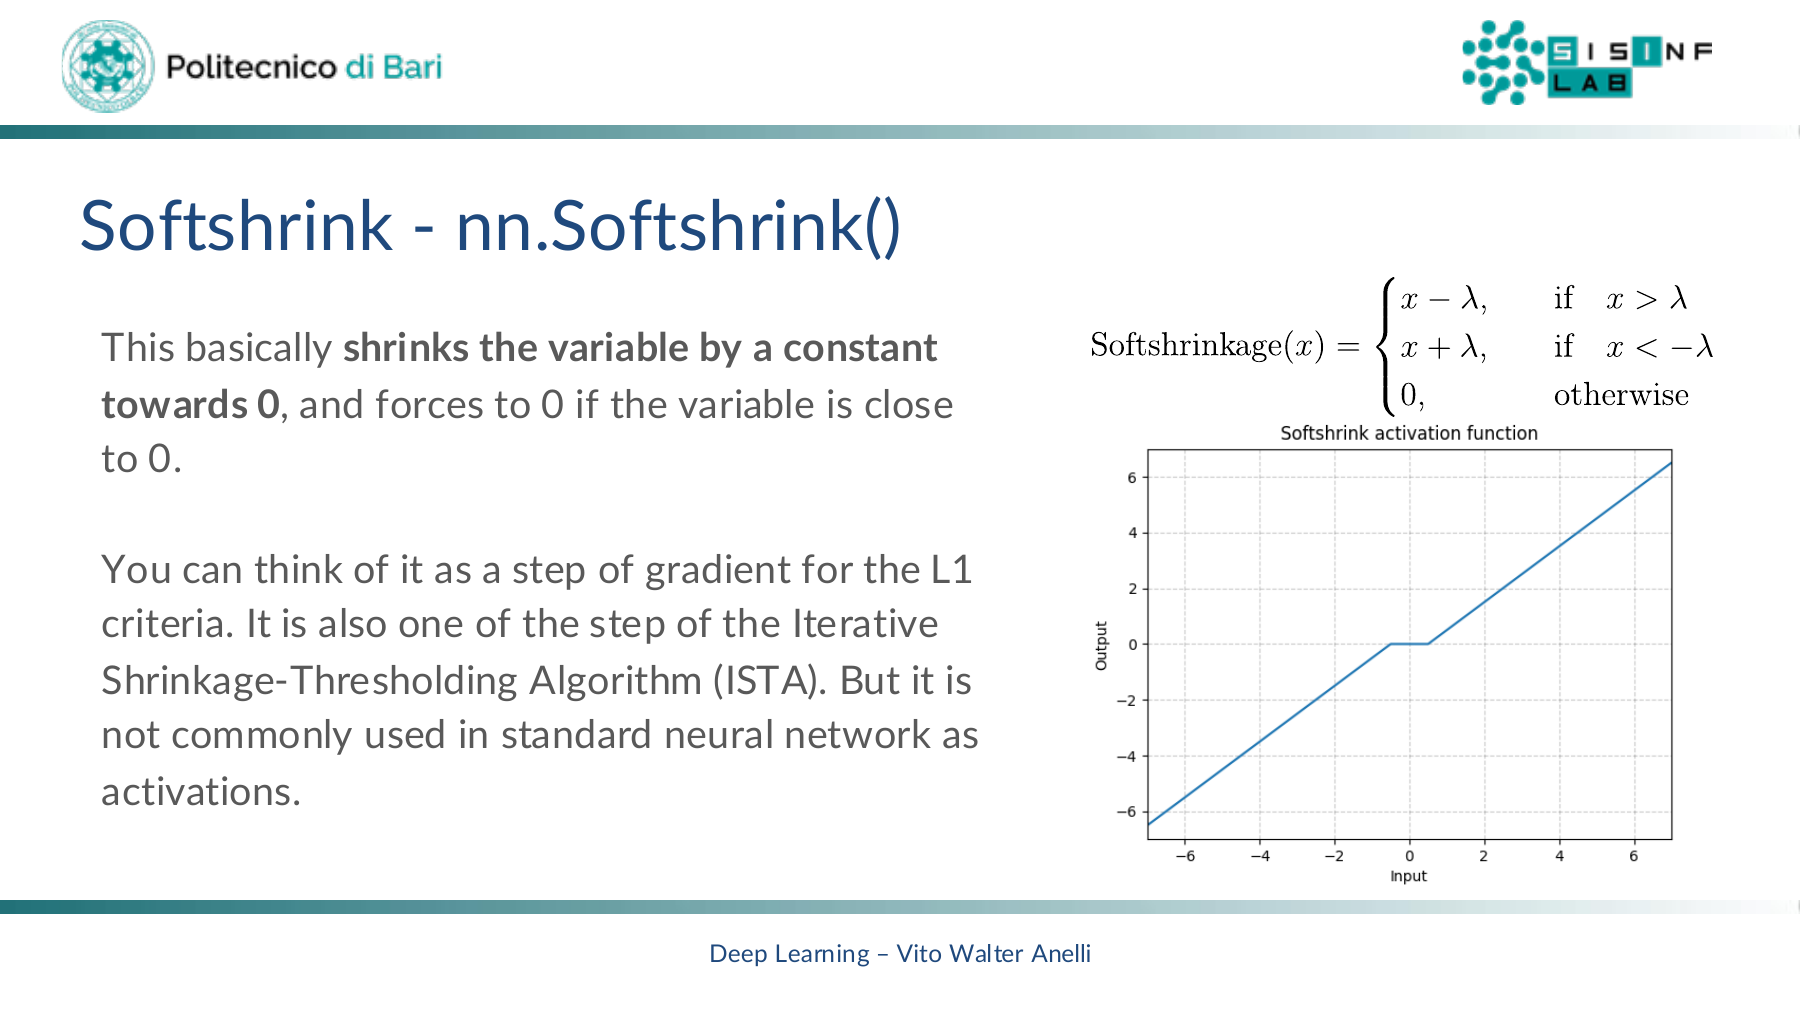
\includegraphics[width=0.85\linewidth]{figures/af03_softshrink.png}
  \caption{Softshrink: riduce il valore assoluto di $x$ di $\lambda$ verso zero,
           forzando a zero gli input nell'intervallo $[-\lambda, \lambda]$.
           Corrisponde a un passo del gradiente per la norma $L_1$ ed è
           uno step dell'algoritmo ISTA (\emph{Iterative Shrinkage-Thresholding}).
           Non è comunemente usata come attivazione nelle reti standard.}
  \label{fig:softshrink}
\end{figure}

\subsection{Hardshrink -- \texttt{nn.Hardshrink()}}
\label{subsec:hardshrink}

\begin{equation}
  \operatorname{Hardshrink}(x) =
  \begin{cases}
    x, & \text{se } x > \lambda \\
    x, & \text{se } x < -\lambda \\
    0, & \text{altrimenti}
  \end{cases}
\end{equation}

\begin{figure}[H]
  \centering
  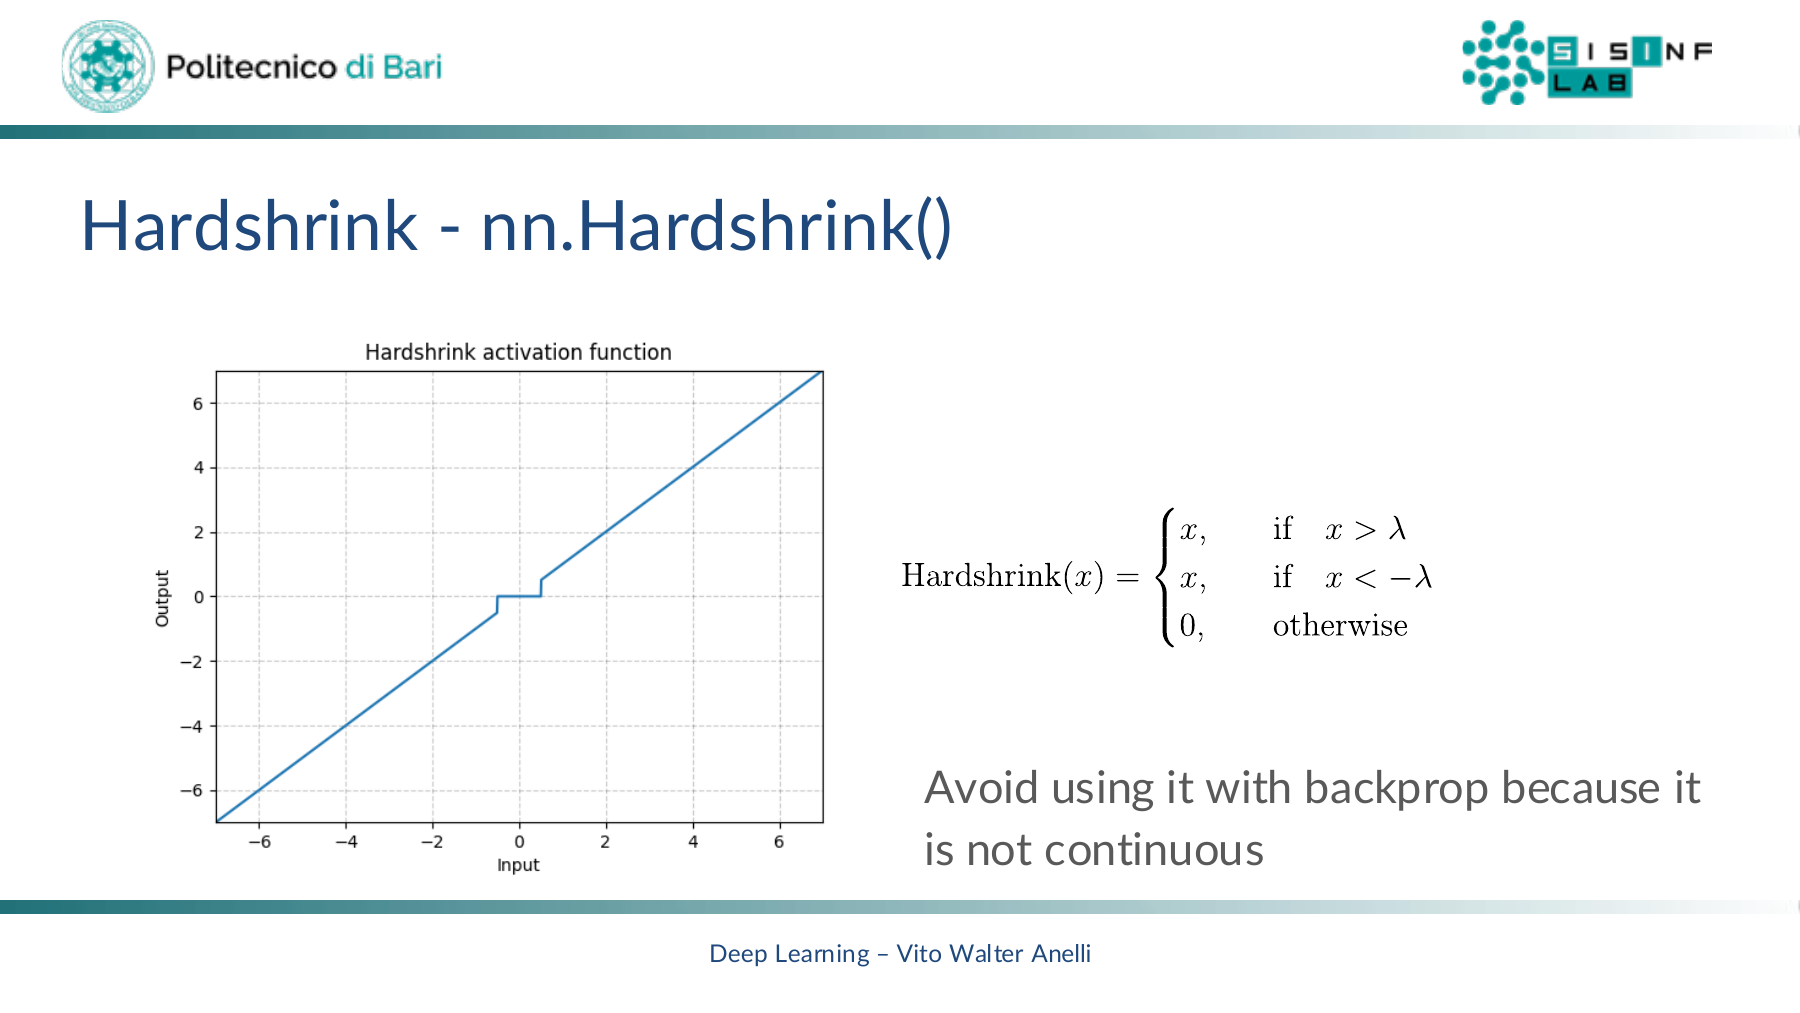
\includegraphics[width=0.85\linewidth]{figures/af03_hardshrink.png}
  \caption{Hardshrink: variante discontinua di Softshrink. La discontinuità in
           $x = \pm\lambda$ rende il gradiente non definito in quei punti, per
           cui \textbf{è sconsigliato l'uso con backpropagation}.
           Utilizzata in alcuni algoritmi di sparse coding fuori dal contesto
           delle reti neurali gradient-based.}
  \label{fig:hardshrink}
\end{figure}

%------------------------------------------------------------
\section{LogSigmoid -- \texttt{nn.LogSigmoid()}}
\label{sec:logsigmoid}

\begin{equation}
  \operatorname{LogSigmoid}(x) = \log\!\left(\frac{1}{1+\exp(-x)}\right).
\end{equation}

\begin{figure}[H]
  \centering
  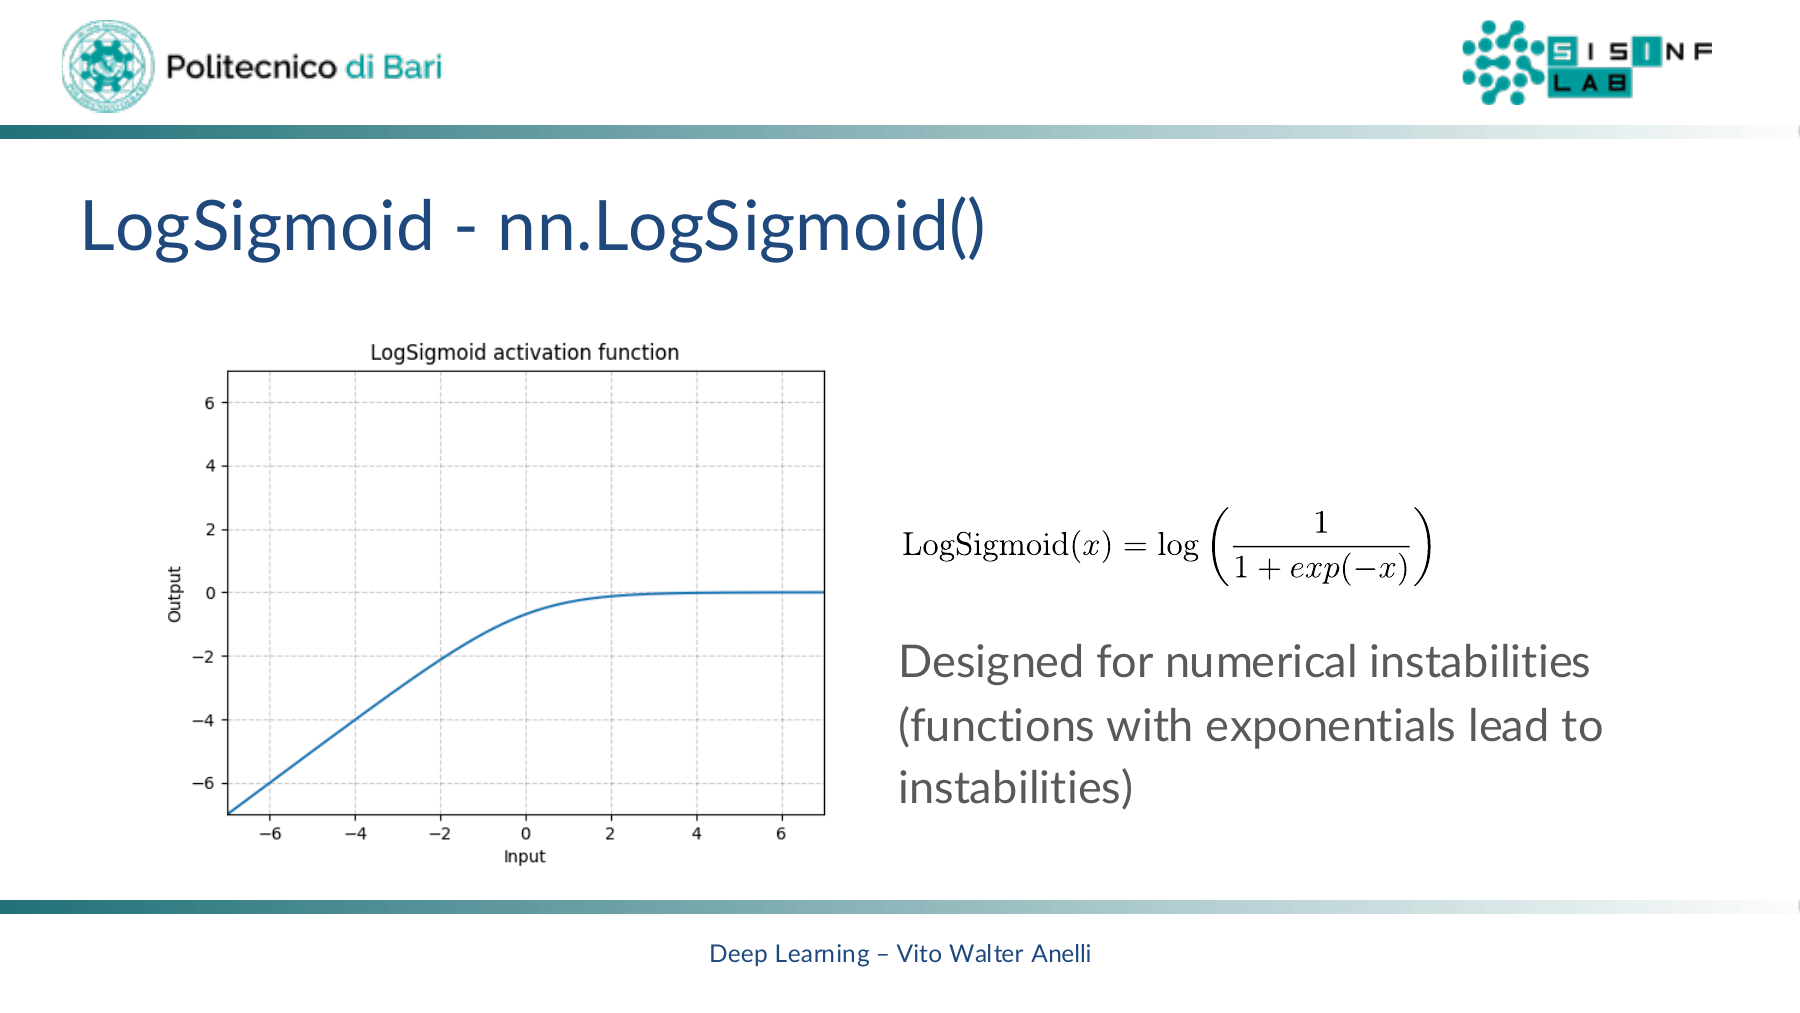
\includegraphics[width=0.85\linewidth]{figures/af03_logsigmoid.png}
  \caption{LogSigmoid: logaritmo della Sigmoid. Progettata per gestire le
           instabilità numeriche che emergono quando funzioni con esponenziali
           vengono composte (overflow/underflow). Usata prevalentemente nelle
           funzioni di costo, non come attivazione interna.}
  \label{fig:logsigmoid}
\end{figure}

%------------------------------------------------------------
\section{Funzioni Vettoriali: Softmin, Softmax, LogSoftmax}
\label{sec:softmax}

Le funzioni di questa sezione agiscono su \textbf{vettori interi}, trasformando
un vettore di scores in una distribuzione di probabilità. Non sono usate come
attivazioni interne, ma tipicamente nell'ultimo layer per compiti di
classificazione multiclasse.

\subsection{Softmin -- \texttt{nn.Softmin()}}
\label{subsec:softmin}

\begin{equation}
  \operatorname{Softmin}(x_i) = \frac{\exp(-x_i)}{\sum_j \exp(-x_j)}.
\end{equation}

\begin{figure}[H]
  \centering
  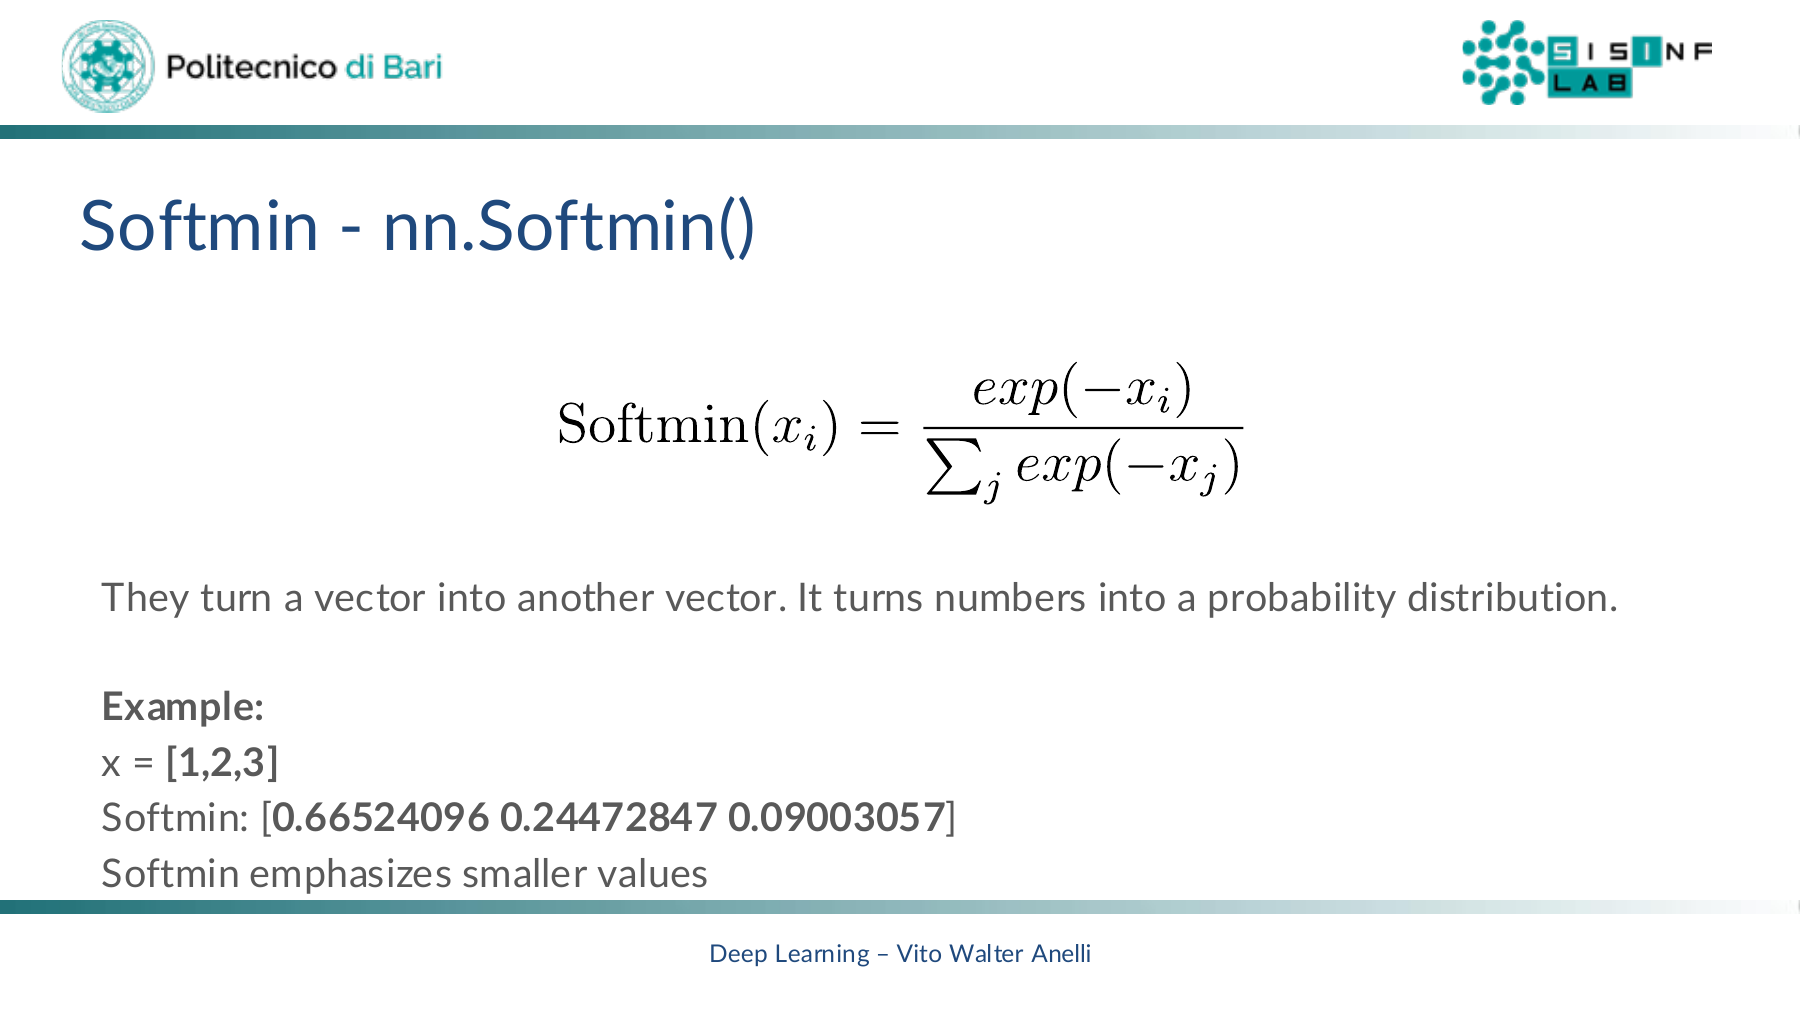
\includegraphics[width=0.72\linewidth]{figures/af03_softmin.png}
  \caption{Softmin: enfatizza i valori più \emph{piccoli} del vettore input.
           Per $x = [1,2,3]$ produce $[0{,}665,\, 0{,}245,\, 0{,}090]$:
           il valore più piccolo ($1$) riceve la probabilità maggiore.
           Raro in pratica; utile in contesti dove si vuole ``selezionare''
           il minimo in modo differenziabile.}
  \label{fig:softmin}
\end{figure}

\subsection{Soft(arg)max -- \texttt{nn.Softmax()}}
\label{subsec:softmax}

\begin{equation}
  \operatorname{Softmax}(x_i) = \frac{\exp(x_i)}{\sum_j \exp(x_j)}.
\end{equation}

\begin{figure}[H]
  \centering
  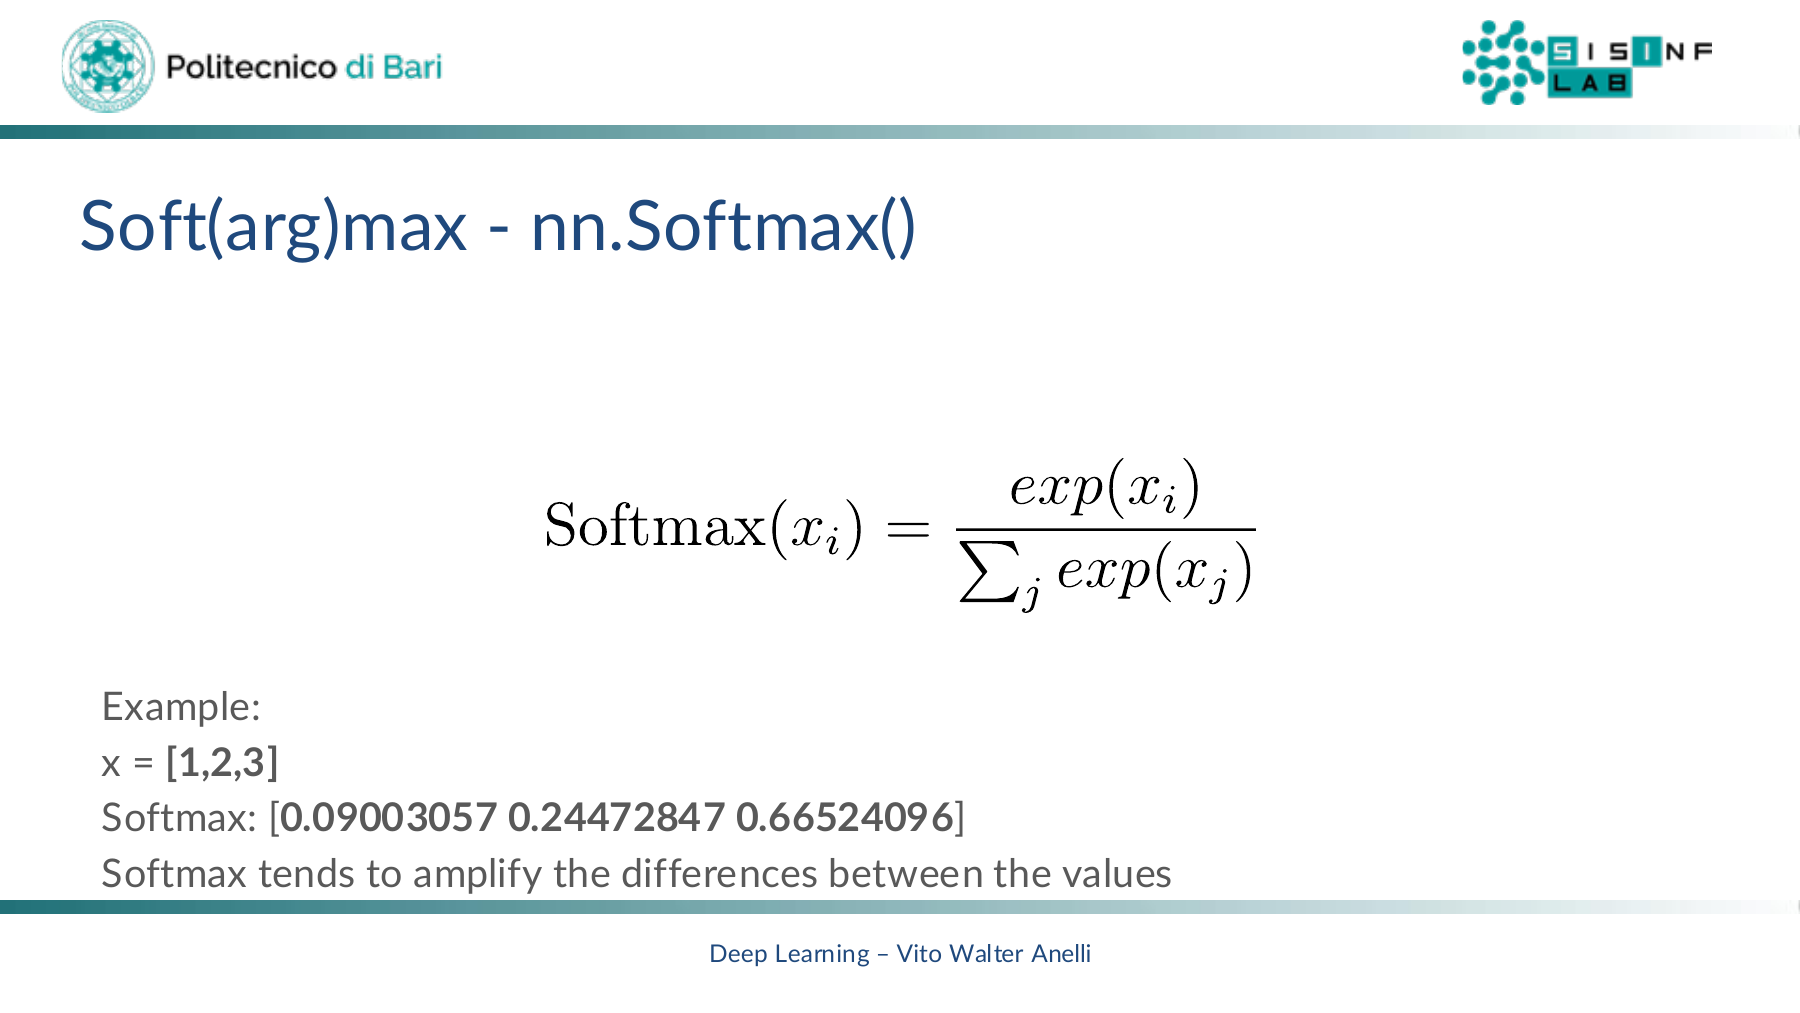
\includegraphics[width=0.72\linewidth]{figures/af03_softmax.png}
  \caption{Softmax: trasforma uno score vettoriale in una distribuzione di
           probabilità sommante a $1$. Enfatizza il valore più grande:
           per $x=[1,2,3]$ produce $[0{,}090,\, 0{,}245,\, 0{,}665]$.
           Amplifica le differenze tra i valori (\emph{winner-takes-all}).}
  \label{fig:softmax}
\end{figure}

\paragraph{Softmax come generalizzazione di Sigmoid.}
La Sigmoid è un caso speciale della Softmax per due classi.
Fissando $x_2 = 0$:

\begin{equation}
  z_1 = \frac{e^{x_1}}{e^{x_1} + e^{x_2}}
      \xrightarrow{x_2=0}
      \frac{e^{x_1}}{e^{x_1} + 1}
      = \frac{1}{1 + e^{-x_1}} = \sigma(x_1).
\end{equation}

\begin{figure}[H]
  \centering
  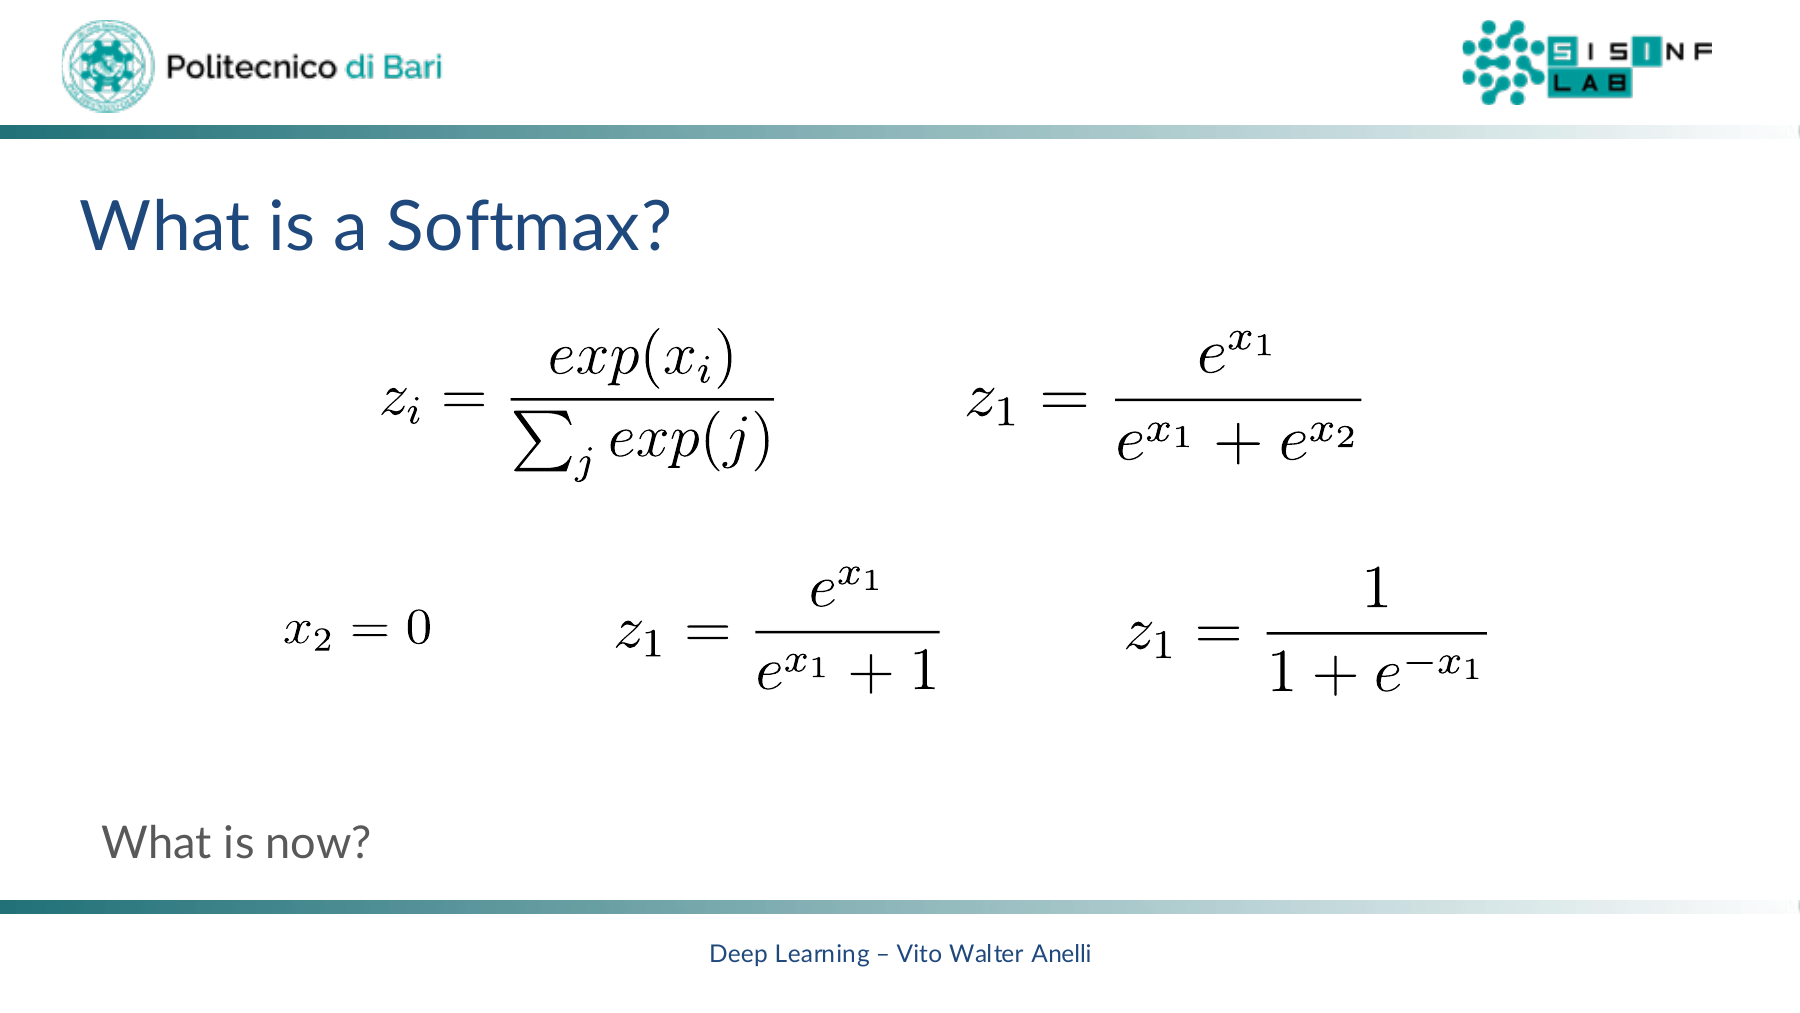
\includegraphics[width=0.72\linewidth]{figures/af03_softmax_relation_sigmoid.png}
  \caption{Derivazione della Sigmoid come caso speciale della Softmax a 2 classi.
           Questa relazione spiega perché la regressione logistica binaria
           (che usa Sigmoid) è un caso speciale della Softmax multiclasse.}
  \label{fig:softmax_relation_sigmoid}
\end{figure}

\subsection{LogSoft(arg)max -- \texttt{nn.LogSoftmax()}}
\label{subsec:logsoftmax}

\begin{equation}
  \operatorname{LogSoftmax}(x_i) = \log\!\left(\frac{\exp(x_i)}{\sum_j \exp(x_j)}\right).
\end{equation}

\begin{figure}[H]
  \centering
  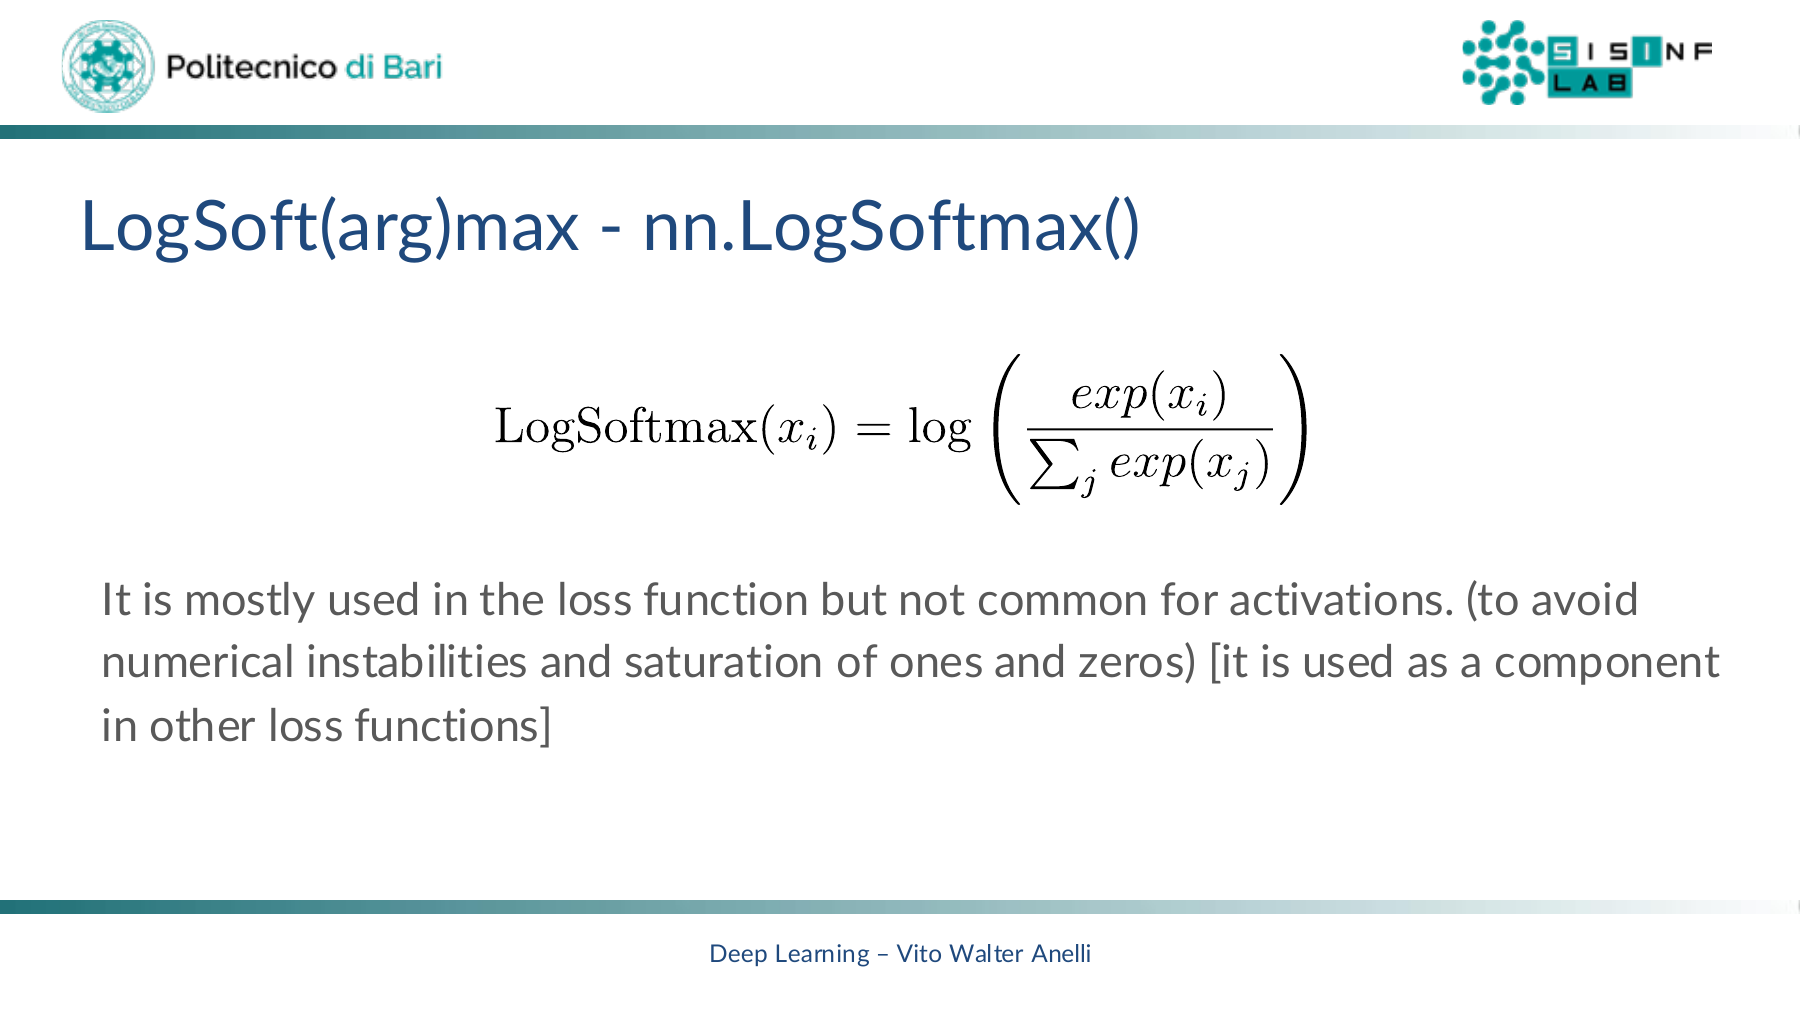
\includegraphics[width=0.72\linewidth]{figures/af03_logsoftmax.png}
  \caption{LogSoftmax: usato principalmente nelle funzioni di costo (es.\ in
           combinazione con \texttt{nn.NLLLoss}) per evitare instabilità
           numeriche (overflow/underflow per esponenziali grandi) e la
           saturazione di valori in $0$ e $1$. Non è comune come attivazione
           interna.}
  \label{fig:logsoftmax}
\end{figure}

%------------------------------------------------------------
\section{Softmax e Cross-Entropy Loss}
\label{sec:softmax-crossentropy}

Nell'ultimo layer di un classificatore multiclasse, la Softmax viene accoppiata
alla \textbf{Cross-Entropy Loss}:

\begin{equation}
  \mathcal{L}_{\mathrm{CE}} = -\sum_i q_i \log(p_i),
\end{equation}
dove $q_i \in \{0,1\}$ è la label one-hot e $p_i = \operatorname{Softmax}(x_i)$.
Per un vettore one-hot, la somma collassa a un solo termine:

\begin{equation}
  \mathcal{L}_{\mathrm{CE}} = -\log\bigl(\operatorname{Softmax}(x_{\mathrm{corr}})\bigr),
\end{equation}
ossia si \emph{massimizza la probabilità assegnata alla classe corretta}
(o equivalentemente si minimizza il suo logaritmo negativo).

\begin{figure}[H]
  \centering
  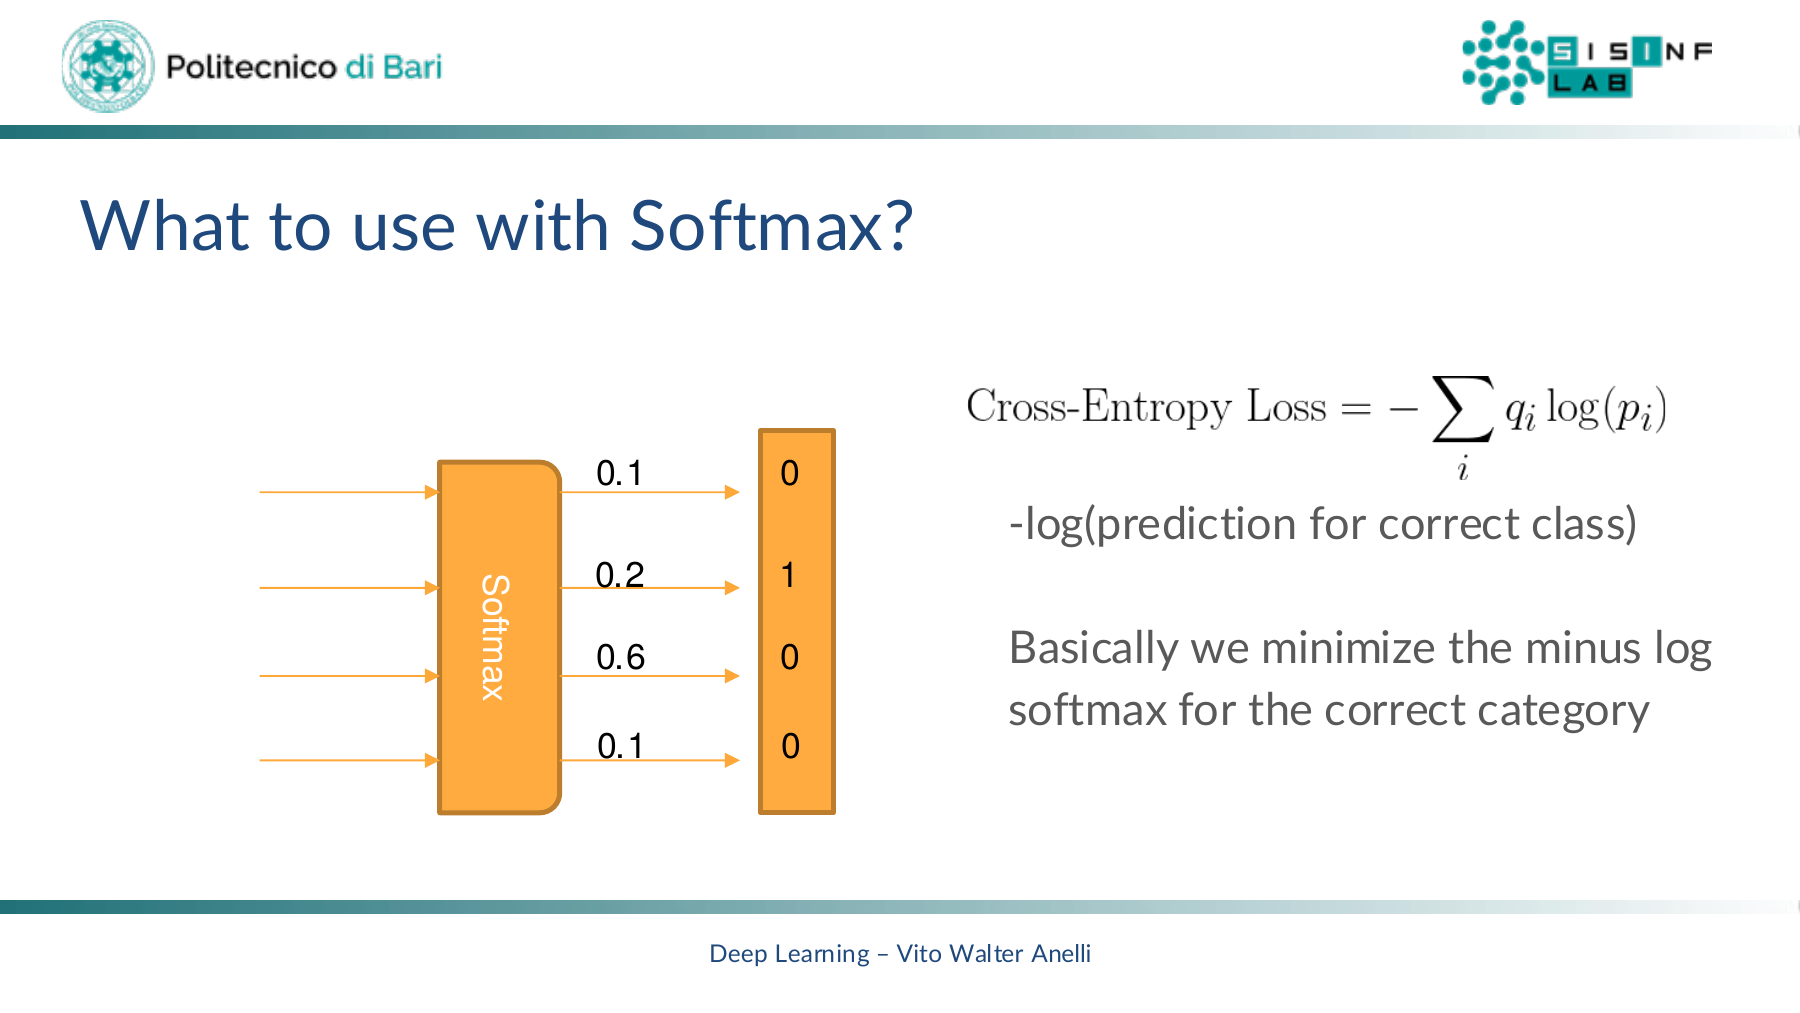
\includegraphics[width=0.82\linewidth]{figures/af03_softmax_crossentropy.png}
  \caption{Softmax + Cross-Entropy Loss: il layer Softmax produce una distribuzione
           $[0{,}1,\ 0{,}2,\ 0{,}6,\ 0{,}1]$ mentre il target one-hot seleziona
           la classe 2 ($[0,1,0,0]$). La loss è $-\log(0{,}2)$. In pratica
           si usa \texttt{nn.CrossEntropyLoss} in PyTorch che fonde
           \texttt{LogSoftmax} e \texttt{NLLLoss} per stabilità numerica.}
  \label{fig:softmax_crossentropy}
\end{figure}

In PyTorch è raccomandato usare \texttt{nn.CrossEntropyLoss} anziché
\texttt{nn.Softmax} + \texttt{nn.NLLLoss} separatamente, perché la
formulazione unificata implementa il log-sum-exp trick che evita overflow
numerici \citep{bishop2024}.

%------------------------------------------------------------
\section{Guida Pratica alla Scelta}
\label{sec:practical-guide}

La scelta della funzione di attivazione dipende dal task, dalla profondità
della rete e dai requisiti computazionali. Le linee guida di \citet{bishop2024}
e del corso NYU-DL possono essere sintetizzate nella Tabella~\ref{tab:activation_guide}.

\begin{table}[H]
  \centering
  \caption{Guida pratica alla scelta della funzione di attivazione.}
  \label{tab:activation_guide}
  \small
  \begin{tabularx}{\linewidth}{l l l X}
    \toprule
    \textbf{Funzione} & \textbf{Output range} & \textbf{Gradiente} & \textbf{Uso tipico} \\
    \midrule
    ReLU       & $[0, +\infty)$                  & Non sat.\ (pos.) & Default hidden layer \\
    Leaky ReLU & $(-\infty,+\infty)$              & Non saturante    & ReLU con dead neurons \\
    PReLU      & $(-\infty,+\infty)$              & Apprendibile     & Quando LReLU è insufficiente \\
    ELU        & $(-\alpha, +\infty)$             & Non saturante    & Hidden, mean $\approx 0$ \\
    SELU       & $(\approx{-1{,}76}, +\infty)$   & Self-norm.       & Reti senza BatchNorm \\
    GELU       & $\approx(-0{,}17, +\infty)$     & Non mon.         & Transformer (BERT, GPT) \\
    Sigmoid    & $(0, 1)$                         & Saturante        & Output prob.\ binaria, gate \\
    Tanh       & $(-1, 1)$                        & Saturante        & RNN, output centrato \\
    Softmax    & $(0,1)^C$, $\sum=1$              & Vettoriale       & Output multiclasse \\
    \bottomrule
  \end{tabularx}
\end{table}

\paragraph{Raccomandazioni operative.}
\begin{enumerate}
  \item \textbf{Punto di partenza}: usare \textbf{ReLU} per i layer nascosti
        di MLP e CNN; è semplice, efficiente e funziona bene nella maggior parte
        dei casi.
  \item \textbf{Dead neurons}: se si osservano molti neuroni inattivi (output
        sempre zero), passare a \textbf{Leaky ReLU} o \textbf{ELU}.
  \item \textbf{Reti senza BatchNorm}: considerare \textbf{SELU}, che fornisce
        self-normalization automatica.
  \item \textbf{Transformer}: preferire \textbf{GELU}, che è la scelta standard
        in BERT, GPT-2/3 e modelli derivati.
  \item \textbf{Output layer}: usare \textbf{Sigmoid} per classificazione binaria,
        \textbf{Softmax} per multiclasse, nessuna attivazione (o ReLU/Softplus)
        per regressione con output positivo.
  \item \textbf{Loss function}: abbinare sempre \texttt{nn.CrossEntropyLoss}
        alla Softmax (fuse internamente con \texttt{LogSoftmax}) per stabilità
        numerica.
\end{enumerate}

%------------------------------------------------------------
\section{Riepilogo}
\label{sec:summary-ch3}

\begin{center}
\small
\begin{tabularx}{\linewidth}{l l X}
  \toprule
  \textbf{Problema} & \textbf{Causa} & \textbf{Soluzione} \\
  \midrule
  Vanishing gradient  & Saturazione Sigmoid/Tanh  & ReLU, ELU, GELU \\
  Dead neurons        & ReLU $=0$ per input neg.  & LReLU, PReLU, ELU \\
  Output non centrato & ReLU $\geq 0$ sempre      & ELU, SELU, BatchNorm \\
  Instabilità num.    & Exp.\ overflow in Softmax & LogSoftmax, CrossEntropyLoss \\
  Parametri extra     & PReLU: $a$ apprendibile   & Beneficio: adattività \\
  Non monotonicità    & GELU ha un ``dip''         & Proprietà regolatrice \\
  \bottomrule
\end{tabularx}
\end{center}

Le funzioni di attivazione rappresentano uno degli assi portanti
dell'ingegneria delle reti neurali: la scelta sbagliata può precludere
l'apprendimento nei layer profondi (vanishing gradient), mentre la scelta
giusta velocizza la convergenza e migliora la generalizzazione.
Il consenso attuale nella letteratura è di usare ReLU o le sue varianti
non saturanti come default, riservando Sigmoid e Tanh ai casi in cui
la struttura del problema lo impone (output probabilistici, meccanismi
di gating, reti ricorrenti).
